%% Placeholder for chapter on linear, quadratic, and geometric models

\section{Linear Programs: An Optimization Problem}
\subsection{Terminology and concepts regarding LP problem}
Consider following problem, i.e., Liner programming with equality and inequity constraints:
\begin{align*}
	\min_{x\in \reals^n}& c^{\trans}x + d\\
	s.t. \quad &Ax = b\\
	&Gx \leq h
\end{align*}

where $x\in \reals^n, c\in \reals^n, d\in \reals, A\in \reals^{q\times n}, b\in \reals^q, G\in \reals^{m\times n}, h\in \reals^m$.

Note that, the function $p(x)=c^{\trans}x + d$ is called the objective function and $x$ is called the decision variable. The goal of this problem is to find $x^*$ such that the optimal value $p^*$ of the objective function is achieved.

This formulation is the general form, and let's write it in matrix form(list of vectors), that is,

$$
A = 
\begin{bmatrix}
\alpha^{(1)^{\trans}}\\
...\\
\alpha^{(q)^{\trans}}
\end{bmatrix}
\qquad	
G = 
\begin{bmatrix}
g^{(1)^{\trans}}\\
...\\
g^{(q)^{\trans}}
\end{bmatrix}
$$

$$<\alpha^{(i)}, x> =b_i,\ i\in \left[q\right]$$
$$<G^{(i)}, x>\leq h_i,\ i\in \left[m\right]$$

Note that, there are also two other forms which are commonly used.

1. Inequality form (only contains inequity constraints)
\begin{align*}
	min \quad &c^{\trans}x+d\\
	s.t. \quad &Gx\leq h\\
\end{align*}
Given the general form, to get the inequality form, we simply break the equality
\begin{equation*}
	Ax = b \Leftrightarrow Ax\geq b, Ax\leq b
\end{equation*}
So we can get inequality form as follows:
\begin{align*}
	\min c^{\trans}x&+d\\
	\qquad s.t. \quad Gx &\leq h\\
	Ax &\leq b\\
	-Ax &\leq -b
\end{align*}

2. Standard form (only contains equality and all variables are non negative)
\begin{align*}
	\min \quad&c^{\trans}x+d\\
	s.t. \quad&Ax = b\\
	&x\geq 0
\end{align*}

Given the general form, we can also convert it into a standard form in 2 steps.

Step 1: Introducing the slack variables $s$

Given the general form,
\begin{align*}
	\min \quad&c^{\trans}x+d\\
	s.t. \quad&Gx\leq h\\
	&Ax = b
\end{align*}
We add the slack variables $s$ so that the formulation become:
\begin{align*}
	\min \quad&c^{\trans}x+d\\
	s.t. \quad&Gx + s = h\\
	&Ax = b\\
	&s\geq 0
\end{align*}
Note that the slack variables $s$ must be non negative here.


Step 2: We break the decision variable $x$ by $x= x^+ - x^-$
\begin{align*}
	\min \quad &c^{\trans}(x^{+} - x^{-})+d\\
	s.t. \quad&G(x^{+} - x^{-}) + s = h\\
	&A(x^{+} - x^{-}) = b\\
	&s\geq 0\\
	&x^{+}\geq 0\\
	&x^{-}\geq 0
\end{align*}


Concepts that are frequently used in LP (and also optimization theory):

(1) Feasible set(or feasible region): The set of points $S$ that are satisfying all the constraints, i.e.,
$$S = \{x\in\reals^{n}|Ax = b, Gx \leq h \}$$

(2) Feasible solution: The points in the feasible set $S$.

(3) Polyhedron: intersection of finite number of half-spaces, i.e.,
$$\{x\in\reals^{n}|Gx\leq h\}$$

(4) Polytope: bounded intersection of finitely many half-spaces.





\vspace{0.5cm}
Let $p^*$ be the optimal value of the given objective function under the constraints, i.e.,
\begin{align*}
	p^* = \min \quad &c^{\trans}x + d\\
	s.t.\quad &Ax = b\\
	&Gx\leq h
\end{align*}

Remarks on "optimal" value $p^*$ of program:
\begin{itemize}
	\item Lowest cost choice amongst all feasible $x$.
	
	\item Possible here is no minimal choice
	
	\item possible no feasible choice
	
	\item $p^*\in \reals$
\end{itemize}

\vspace{0.5cm}
Let $x^*$ be the optimal choice of the decision variable $x$, i.e.,
\begin{align*}
	x^* = \arg \min \quad&c^{\trans}x + d\\
	s.t.\quad &Ax = b\\
	&Gx\leq h
\end{align*}

Remarks on "optimal" solution $x^*$ of program:
\begin{itemize}
	\item Sometimes $x^*$ does not exist
	
	\item If exists, may not be unique
	
	\item $x^*\in \reals^n$
\end{itemize}




\vspace{0.5cm}
Let's consider an example:\\

During the The Second World War, the US army is considering how to make their soldiers have enough nutrients...\\

Different nutrients in different foods and daily requirement:
\begin{center}
	\begin{tabular}{|c|c|c|c|}
		\hline 
		Nutrients&Meat&Potatoes&Daily Requirement\\
		\hline  
		Carbohydrates&40&200&400\\
		\hline  
		Protein&100&20&200\\
		\hline  
		Fiber&5&40&40\\
		\hline 
	\end{tabular}
\end{center}


\vspace{0.3cm}
The price of meat and potatoes:
\begin{center}
	\begin{tabular}{|c|c|}
		\hline 
		Resources&cost/kg\\
		\hline  
		Meat &\$ 1\\
		\hline 
		Potatoes &\$ 0.25\\
		\hline 
	\end{tabular}
\end{center}

Let $x_1$ denotes meat(kg) and $x_2$ denotes potatoes(kg), and we formulate this LP as follows:

Objective function:
\begin{equation*}
	\min_{x_1, x_2} x_1 + \frac{1}{4}x_2 = 
	\min_{x_1, x_2}
	\begin{bmatrix}
		1 & \frac{1}{4}
	\end{bmatrix}
	\begin{bmatrix}
		x_1\\
		x_2
	\end{bmatrix}
\end{equation*}

Constrains:
\begin{align*}
	40x_1 + 200x_2 &\geq 400\\
	100x_1 + 20x_2 &\geq 200\\
	5x_1 + 40x_2 &\geq 40\\
	x_1 \geq 0\\
	x_2 \geq 0
\end{align*}


Rewrite it as $Gx\leq h$, that is,
\begin{equation*}
	\begin{bmatrix}
		-\frac{1}{5} & -1\\
		-\frac{1}{8} & -1\\
		-5 & -1\\
		-1 & 0\\
		0 & -1
	\end{bmatrix}
	\begin{bmatrix}
		x_1\\
		x_2
	\end{bmatrix}\leq
	\begin{bmatrix}
		-2\\
		-1\\
		-10\\
		0\\
		0
	\end{bmatrix}
\end{equation*}

\begin{figure}
	\centering
	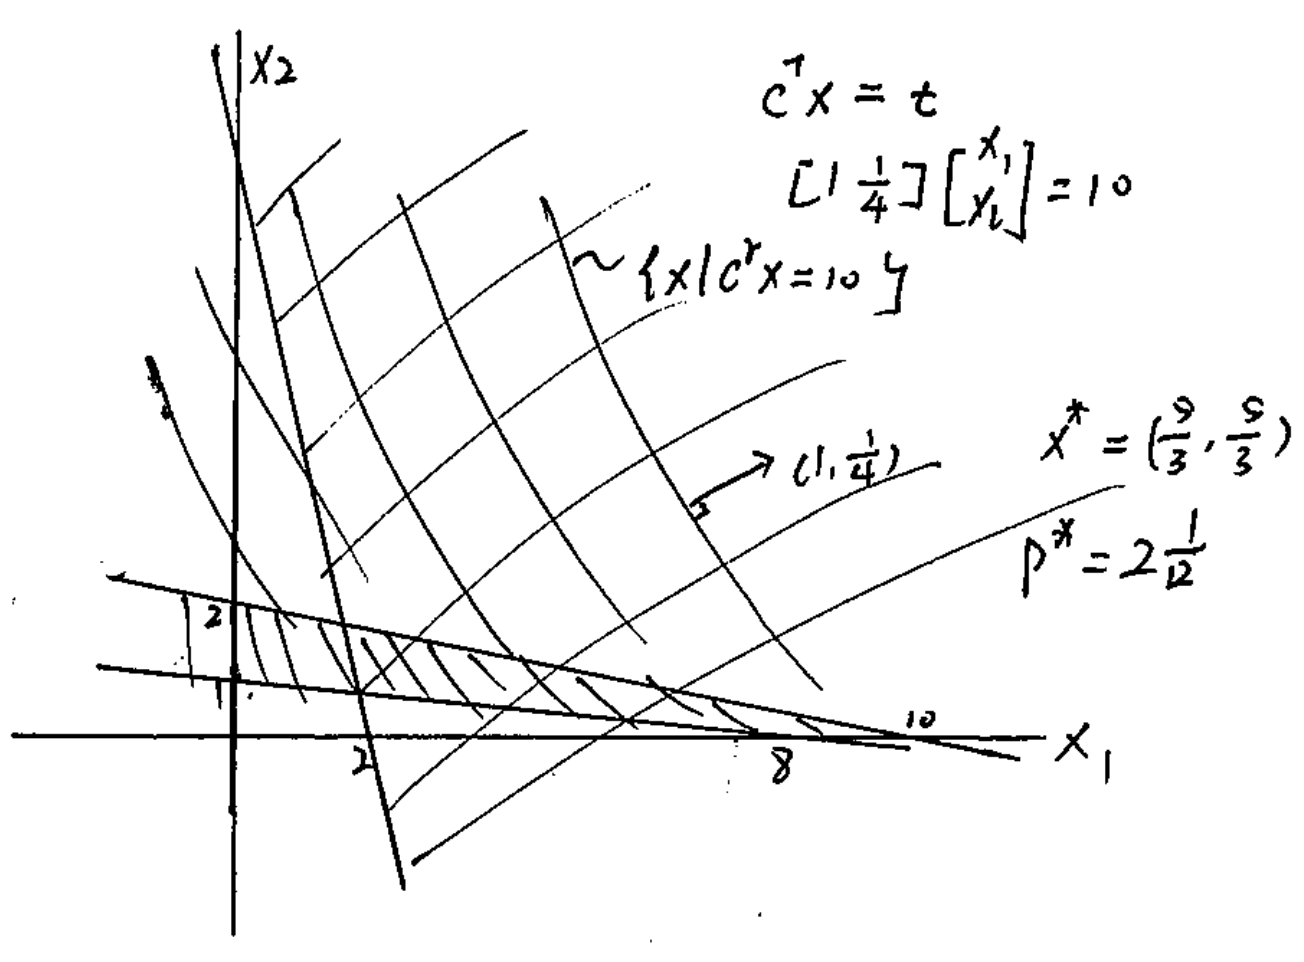
\includegraphics[width=2.1in,height=2.1in]{figures/ch06/figure5.png}
	%\caption{This is an inserted JPG graphic} 
	%\label{fig:graph} 
\end{figure}



\subsection{LP without constraints}

Consider the LP does not have constraints, so we have
\begin{align*}
	p^* &= \min c^{\trans}x+d\\
	x^* &= \arg \min_{x\in \reals^n} \quad c^{\trans}x+d
\end{align*}

\vspace{0.5cm}
Situation 1: $c = 0 \in \reals^n$
\begin{align*}
	p^* &= \min_{x\in \reals^n} \quad d=d\\
	x^* &= \arg \min_{x\in \reals^n} \quad d = \reals^n
\end{align*}

Situation 2: $c \neq 0 \in \reals^n$
\begin{align*}
	p^* &= -\infty\quad \text{by convention if no minimum}\\
	x(\alpha) &= -\alpha c \quad \alpha \geq 0\\
	c^{\trans}x + d &= c^{\trans}(-\alpha c) + d = \alpha - \alpha c^{\trans}c = \alpha - \alpha\Vert c\Vert^2_2\\
	x^* &\text{doesn't exist}
\end{align*}

Thus, for unconstrained LP we conclude that
$$
%\label{eq6}
p^*=\left\{
\begin{aligned}
d &  & \text{if } c=0 \\
-\infty &  & \text{otherwise}
\end{aligned}
\right.
%\label{eq6}
\qquad
x^*=\left\{
\begin{aligned}
\reals^n & &\text{if } c=0 \\
\text{doesn't exist} &  & \text{otherwise}
\end{aligned}
\right.
$$

Let's think about the geometry of cost function:
$$
F_0(x) =c^{\trans}x + d
$$
where $F_0(x)$ is the objective function and it turns out that it is also an affine function.

Recall that the level set for $F_0(x)$, 
\begin{align*}
	c_{F_0}(t) &=\{ x\in \reals^n | F_0(x) = c^{\trans}x + d = t \}\\
	&= \{x\in \reals^n | C^{\trans}x = (t-d) \}
\end{align*}

Obviously, the level set for $F_0(x)$ defines a hyperplane, and when $t=d$ it defines a subspace(go through the origin). Let's consider two level sets, for $t_1$ and $t_2$,

\begin{figure}
	\centering
	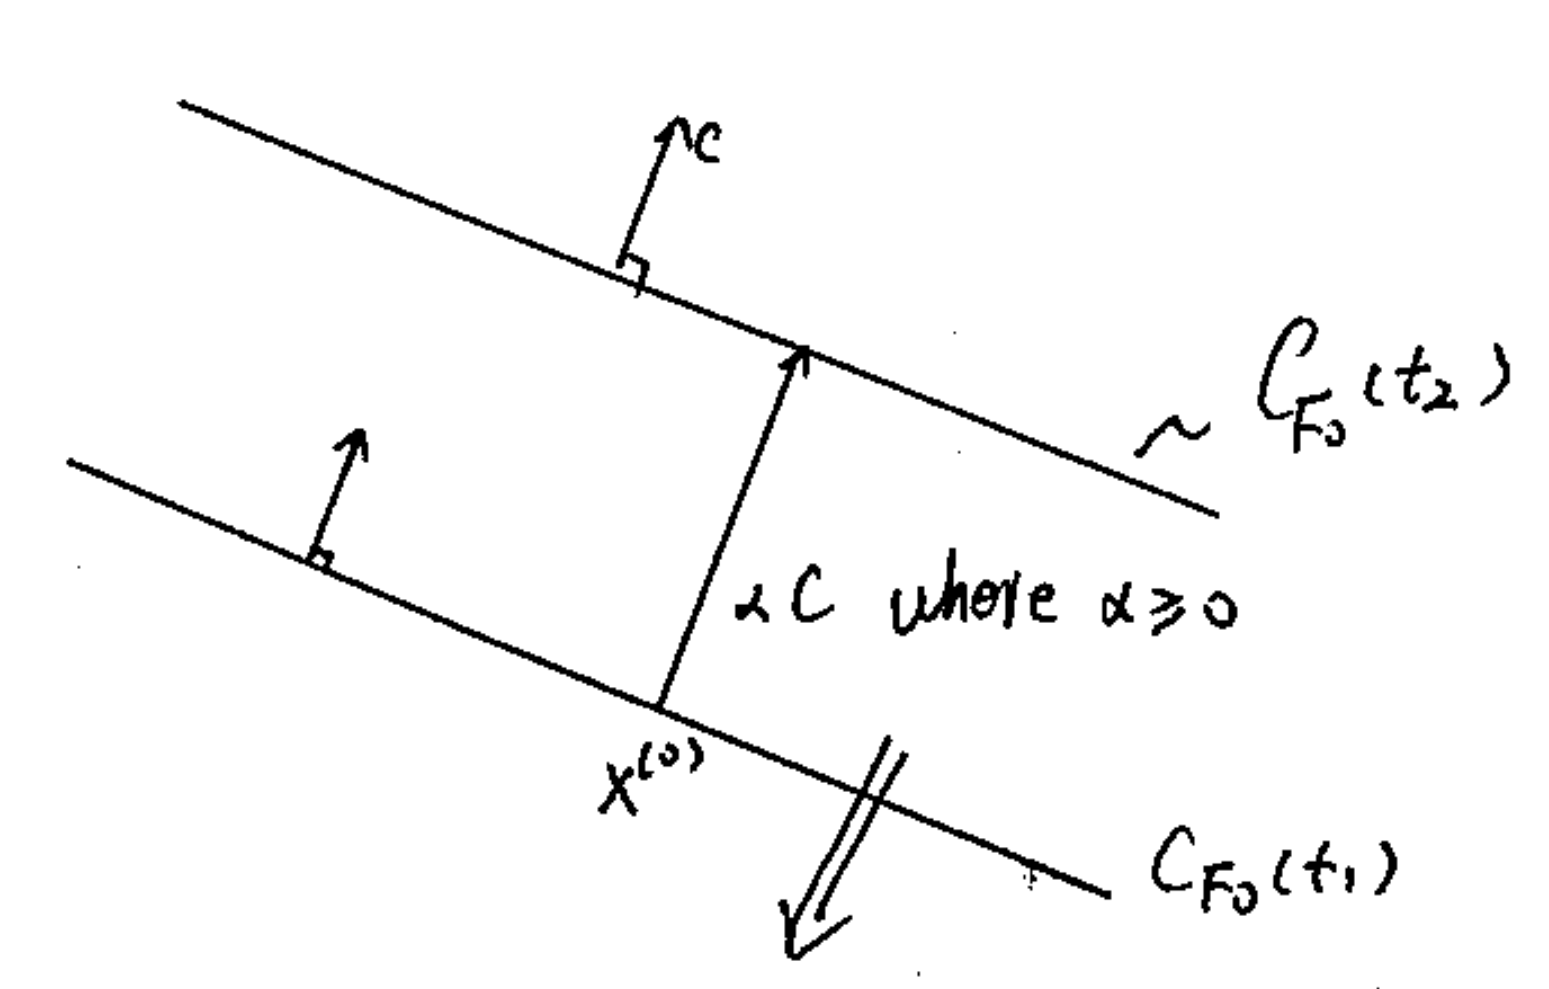
\includegraphics[width=2.1in,height=2.1in]{figures/ch07/figure1012_1.png}
	%\caption{This is an inserted JPG graphic} 
	%\label{fig:graph} 
\end{figure}

Note that $c$ is the normal vector to $x$. Let's find the relationship between $t_1$ and $t_2$:

Approach (1)
\begin{align*}
	t_2 &= c^{\trans}(x^{(0)}+\alpha c) + d\\
	t_1 &= c^{\trans}x^{(0)} + d\\
	t_2 - t_1 &= [c^{\trans}x^{(0)} + d + \alpha \Vert c\Vert ^2] - c^{\trans}x^{(0)} = \alpha \Vert c \Vert^2
\end{align*}
So apparently $t_2>t_1$.

Approach (2)
\begin{equation*}
	\nabla F_0(x) =
	\begin{bmatrix}
		\frac{\sigma}{\sigma x_1}(c^{\trans}x+d)\\
		\vdots\\
		\frac{\sigma}{\sigma x_n}(c^{\trans}x+d)
	\end{bmatrix} = 
	\begin{bmatrix}
		c_1\\
		c_2\\
		\vdots\\
		c_n
	\end{bmatrix} = c
\end{equation*}

The gradient points out that the direction of $c$ is the direction of increase in $F_0(x)$. In fact, we could show that the direction of the gradient evaluated at a certain point, is the direction that the value of function increases more rapidly(remind yourself what you have learned in Calculus).

Hence, to minimize the objective function, we go in opposite direction of the gradient, that is, we should go as far as possible along the direction of $-c$ (unless $c=0$).


\vspace{0.5cm}
Now, let's turn back to LP with following constraints as we specified before:
\begin{align*}
	Ax &= b\\
	Gx &\leq h
\end{align*}

Interesting results and interpretation for these two kind of constraints:

(1) $Ax=b$ (Equality constraints): force $x^*$ into an affine set
$$\{x\in \reals^n|Ax = b \} =  \cap^q_{i=1}\{x\in \reals^n|<\alpha^{(i)}, x> = b_i \}$$

(2) $Gx\leq h$ (Inequality constraints): force $x^*$ to be in an intersection of half-spaces
$$\{x\in \reals^n|Gx \leq h \} =  \cap^q_{i=1}\{x\in \reals^n| <g^{(i)}, x> \leq h_i \}$$

(3) The feasible set: intersection of half-spaces and hyperplanes
$$
S = \left(\cap^q_{i=1}\{x\in \reals^n | <\alpha^{(i)}, x> = b_i \}\right) \cap \left(\cap^m_{i=1}\{x\in \reals^n | <g^{(i)}, x> \leq h_i \}\right)
$$


A few remarks:
\begin{itemize}
	\item Concepts of polyhedron and polytope.
	
	\item Ax = b $\rightarrow$ $Ax \leq b$, $Ax \geq b$
\end{itemize}



\begin{example}
	\begin{align*}A &= 
		\begin{bmatrix}
			1 & 1
		\end{bmatrix}
		b = 
		\begin{bmatrix}
			2
		\end{bmatrix}\\
		G &= 
		\begin{bmatrix}
			-1 & 0\\
			0 & -1
		\end{bmatrix}
		h = 
		\begin{bmatrix}
			0\\
			0
		\end{bmatrix}\\
		Ax &= b \rightarrow x_1 + x_2 = 2\\
		Gx &\leq h \rightarrow x_1 \geq 0, x_2\geq 0
	\end{align*}
	
	
	\begin{figure}
		\centering
		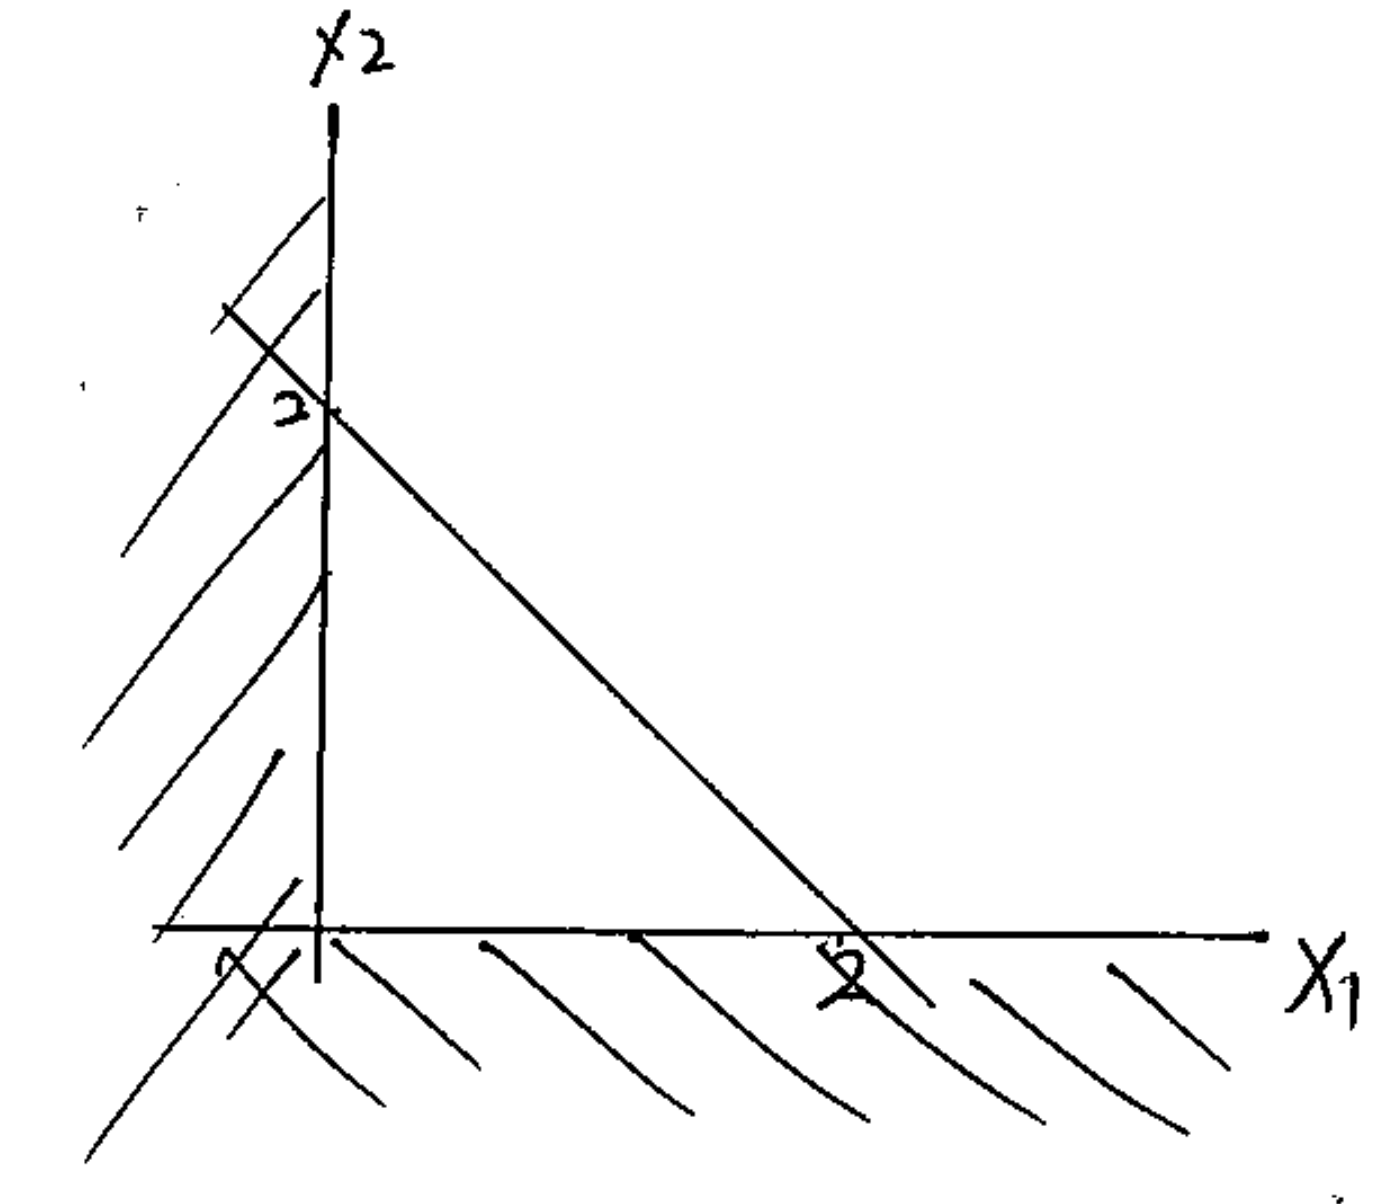
\includegraphics[width=2.1in,height=2.1in]{figures/ch07/figure1012_2.png}
		%\caption{This is an inserted JPG graphic} 
		%\label{fig:graph} 
	\end{figure}
\end{example}








\begin{example}
	Generally, equality constraints move you from a higher dimensional geometry in $\reals^n$ to a slice, which is a lower dimensional geometry. See the following example of losing 1 dimension per linearly independent constraint:
	
	
	\begin{align*}
		A =
		\begin{bmatrix}
			1&1&1
		\end{bmatrix}
	\end{align*}
	\begin{equation*}
		B= 
		\begin{bmatrix}
			1\\
		\end{bmatrix}
	\end{equation*}
	
	\begin{figure}
		\centering
		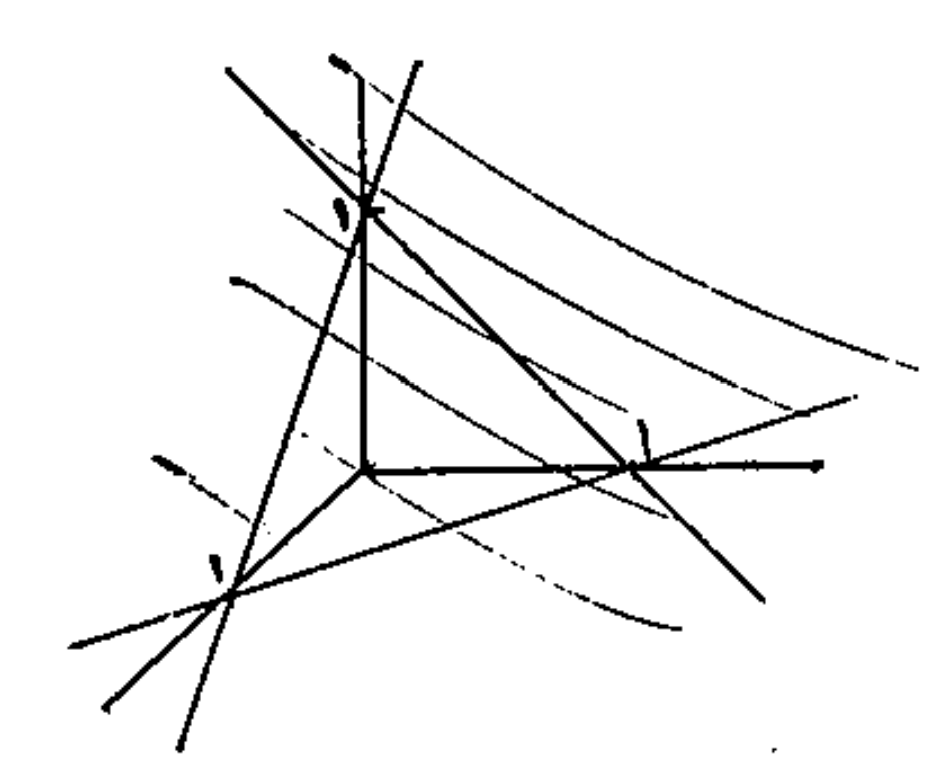
\includegraphics[width=2.1in,height=2.1in]{figures/ch07/figure1012_3.png}
		%\caption{This is an inserted JPG graphic} 
		%\label{fig:graph} 
	\end{figure}
\end{example}

\begin{example}
	In some cases, there may be no intersection between hyperplane:
	
	\begin{equation*}
		\begin{bmatrix}
			1&1\\
			1&1
		\end{bmatrix}
		\begin{bmatrix}
			x_1\\
			x_2
		\end{bmatrix}=
		\begin{bmatrix}
			1\\
			2
		\end{bmatrix}
	\end{equation*}
	
	\begin{figure}
		\centering
		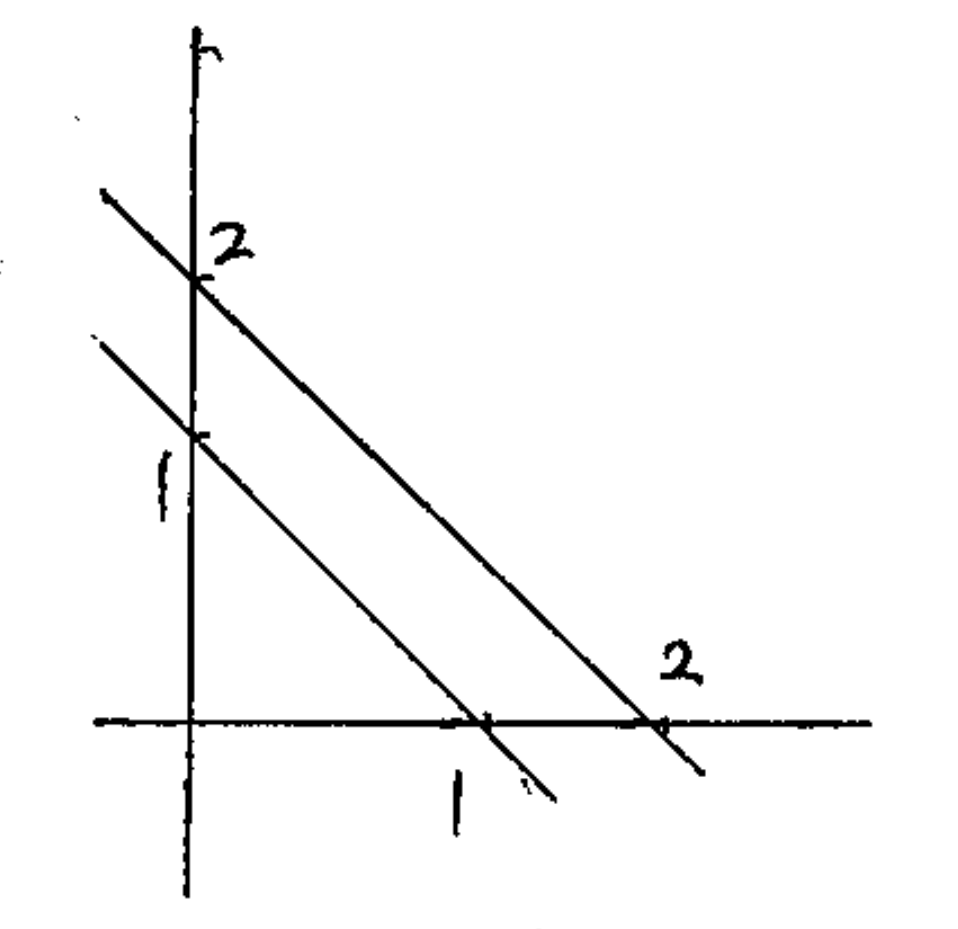
\includegraphics[width=2.1in,height=2.1in]{figures/ch07/figure1012_4.png}
		%\caption{This is an inserted JPG graphic} 
		%\label{fig:graph} 
	\end{figure}
	So the  feasible set is empty, $S = \emptyset$.
	
	\vspace{0.3cm}
	This situation may also happen with inequalities constraints:
	\begin{align*}
		\begin{bmatrix}
			-1&0\\
			1&0
		\end{bmatrix}
		\begin{bmatrix}
			x_1\\
			x_2
		\end{bmatrix}&\leq
		\begin{bmatrix}
			0\\
			-1
		\end{bmatrix}\\
		S &= \emptyset
	\end{align*}
	
\end{example}



\begin{example}
	Generally, to facilitate sketch will often just sketch inequity constraints:
	
	\begin{align*}
		\begin{bmatrix}
			-1 & 0\\
			0 & -1\\
			\frac{1}{2} & -1\\
			1 & 1
		\end{bmatrix}
		\begin{bmatrix}
			x_1\\
			x_2
		\end{bmatrix}
		&\leq 
		\begin{bmatrix}
			0\\
			0\\
			1\\
			3
		\end{bmatrix}\\
	\end{align*}
	
	So we have
	$$x_1 \geq 0$$
	$$x_2 \geq 0$$
	$$x_2 \geq -1 + \frac{1}{2}x_1$$
	$$x_2 \leq 3 - x_1$$
	
	Sketch the feasible set:
	
	\begin{figure}
		\centering
		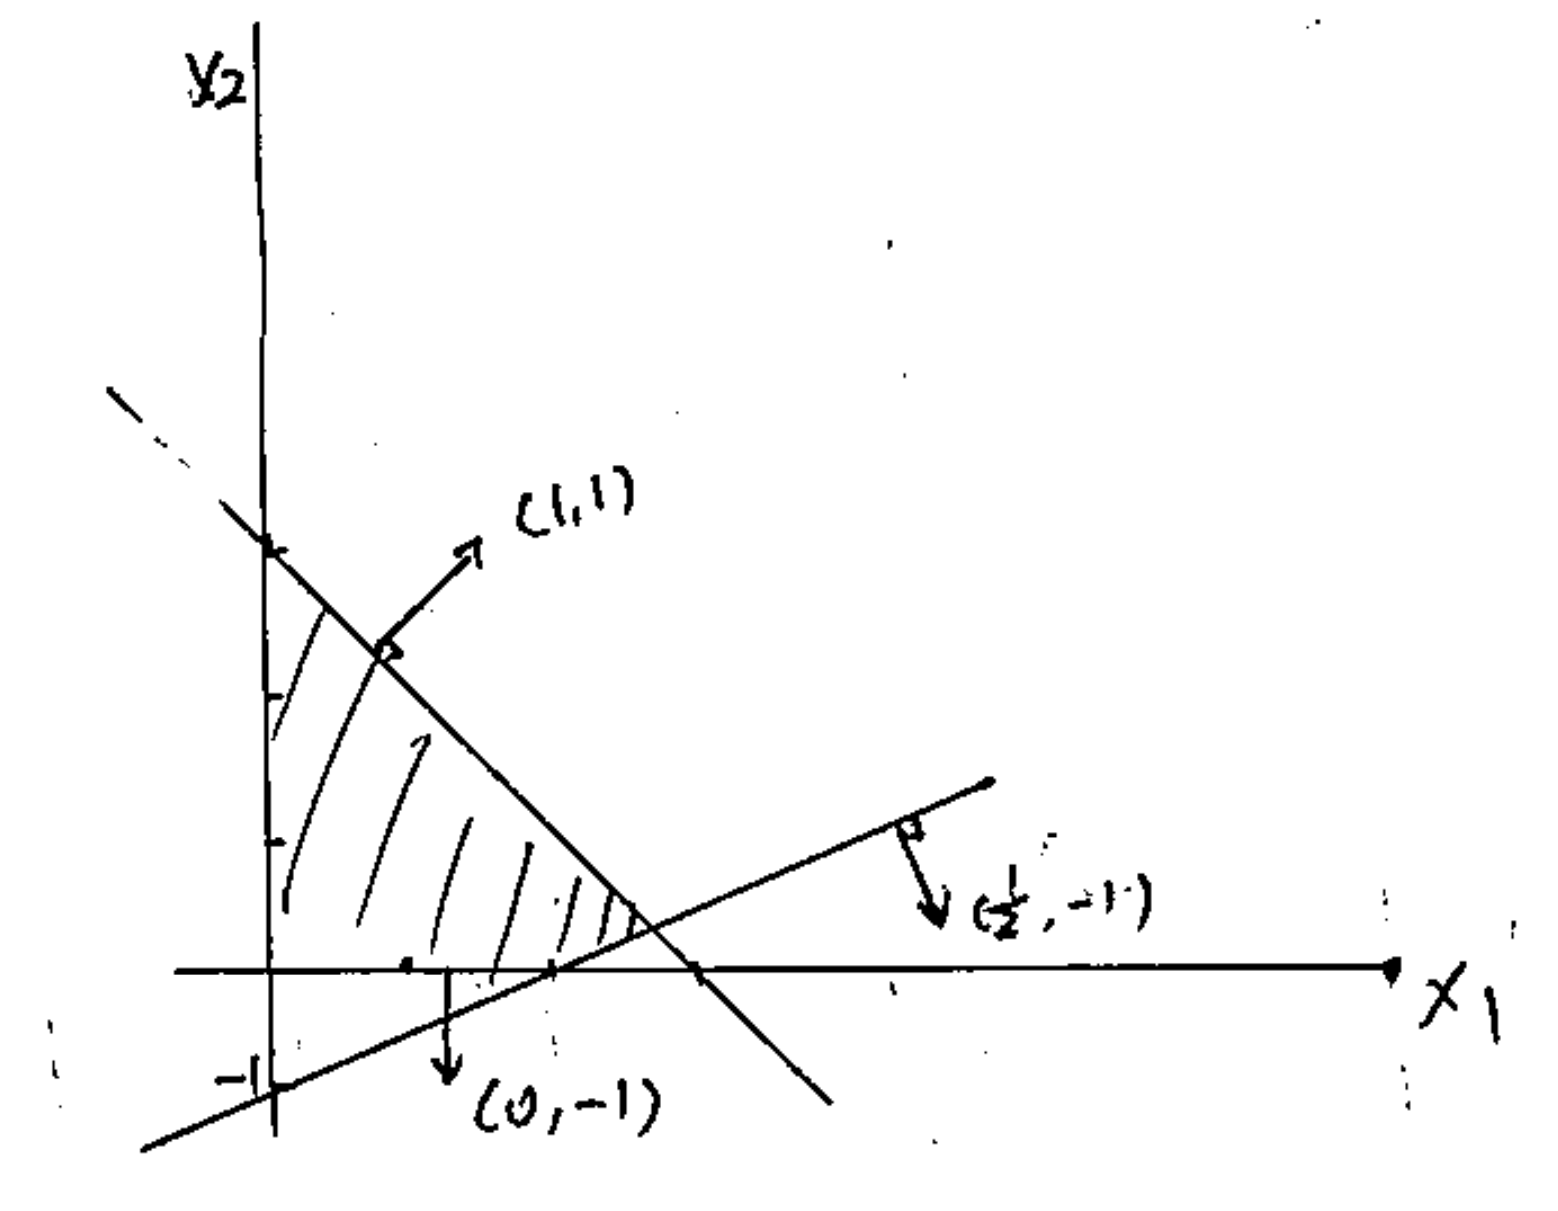
\includegraphics[width=2.1in,height=2.1in]{figures/ch07/figure1012_5.png}
		%\caption{This is an inserted JPG graphic} 
		%\label{fig:graph} 
	\end{figure}
\end{example}

The rows of matrix $G$ are the normal directions of the hyperplanes that define the half-spaces, and the normal directions point outward from the feasible set.


\begin{example}
	Let's combine all these things together, liner objective function, linear equality constraints and linear inequity constraints.
	
	\begin{figure}
		\centering
		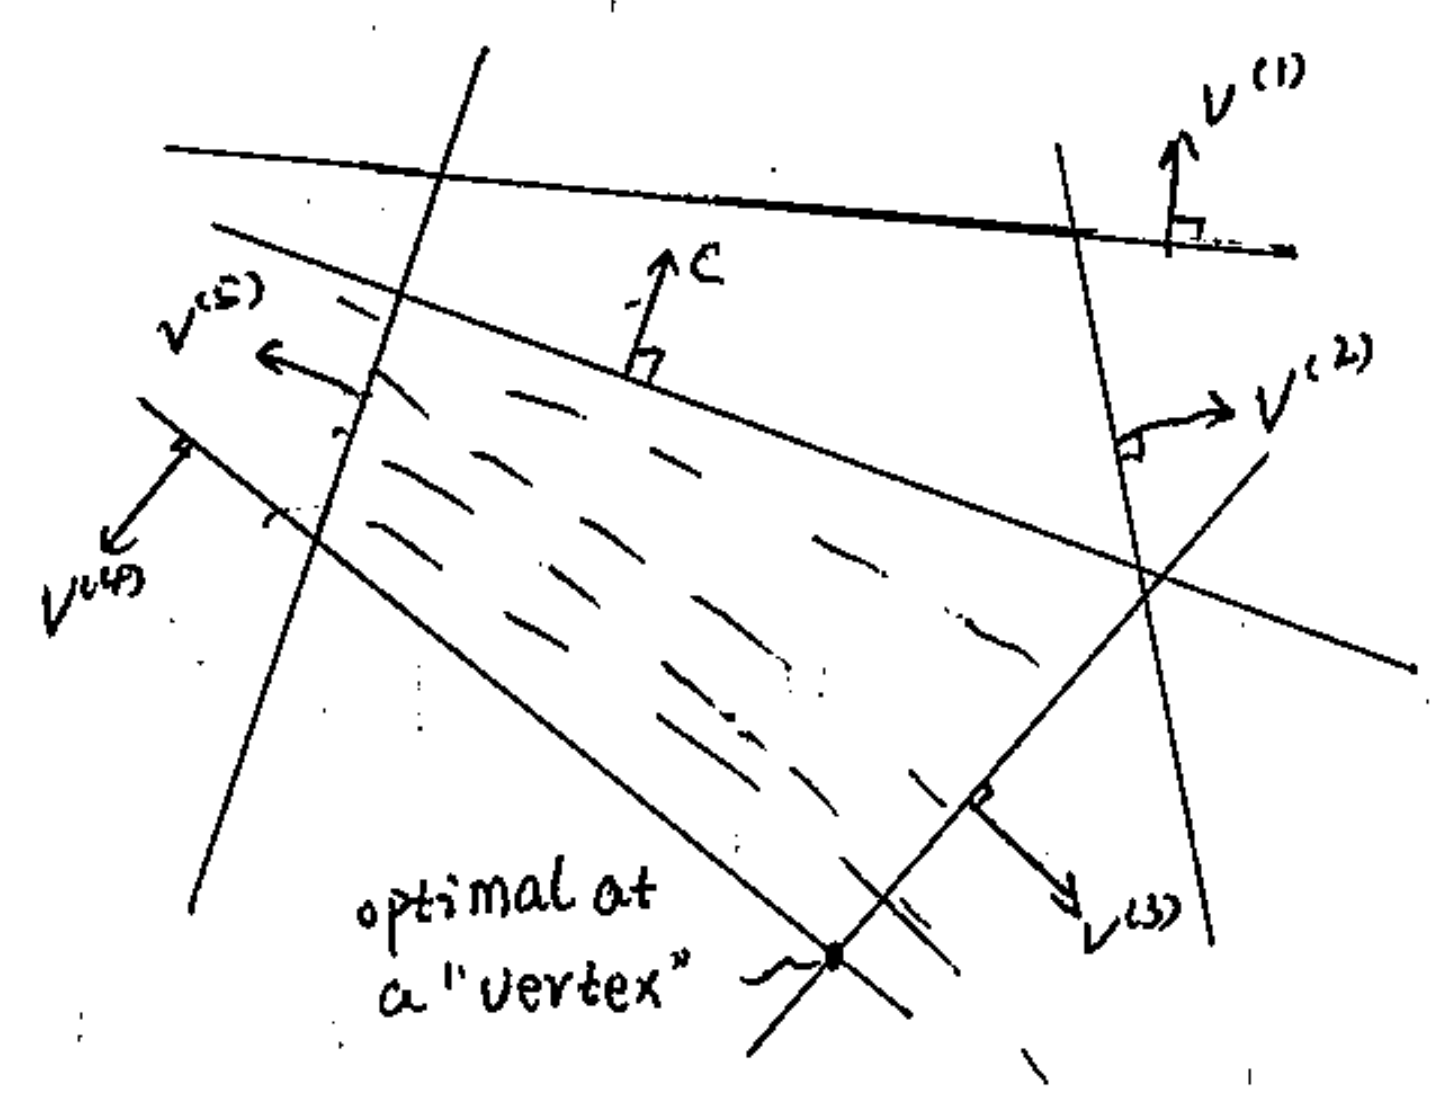
\includegraphics[width=2.1in,height=2.1in]{figures/ch07/figure1012_6.png}
		%\caption{This is an inserted JPG graphic} 
		%\label{fig:graph} 
	\end{figure}
	
	What's optimum? Looks like $x^*=v^{(3)}$.
	
	
	\vspace{0.5cm}
	We may also have a facet with the feasible set 
	$$S = \{x\in \reals^3 | x_1 +x_2+x_3 = 1, x_1 \geq 0, x_2\geq 0,x_3\geq 0\}$$
	
	
	\begin{figure}
		\centering
		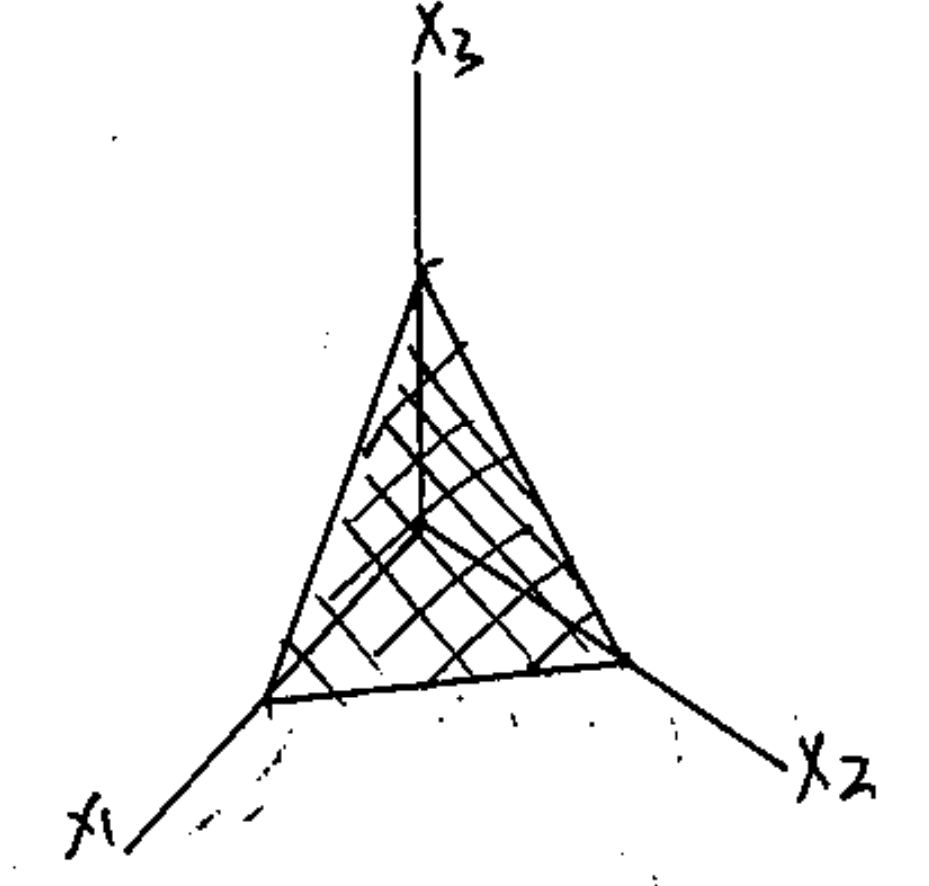
\includegraphics[width=2.1in,height=2.1in]{figures/ch07/figure1012_7.png}
		%\caption{This is an inserted JPG graphic} 
		%\label{fig:graph} 
	\end{figure}
	
	So there are various possibilities here for $p^*$ and  $x^* $:
	
	\begin{itemize}
		\item 1) $x^*$ is unique, $p^*$ finite
		
		\item 2) $x^*$ is not unique, $p^*$ finite. 
		
		\item 3) There is no $x^*$:
		
		\quad a) $S = \emptyset$ (Feasible set is empty), constraint $p^* = \infty$. So we say that this LP problem is infeasible.
		
		\quad b) $S$ is unbounded \& no minimum, constraint $p^* = -\infty$
	\end{itemize}
	
	
	\begin{figure}
		\centering
		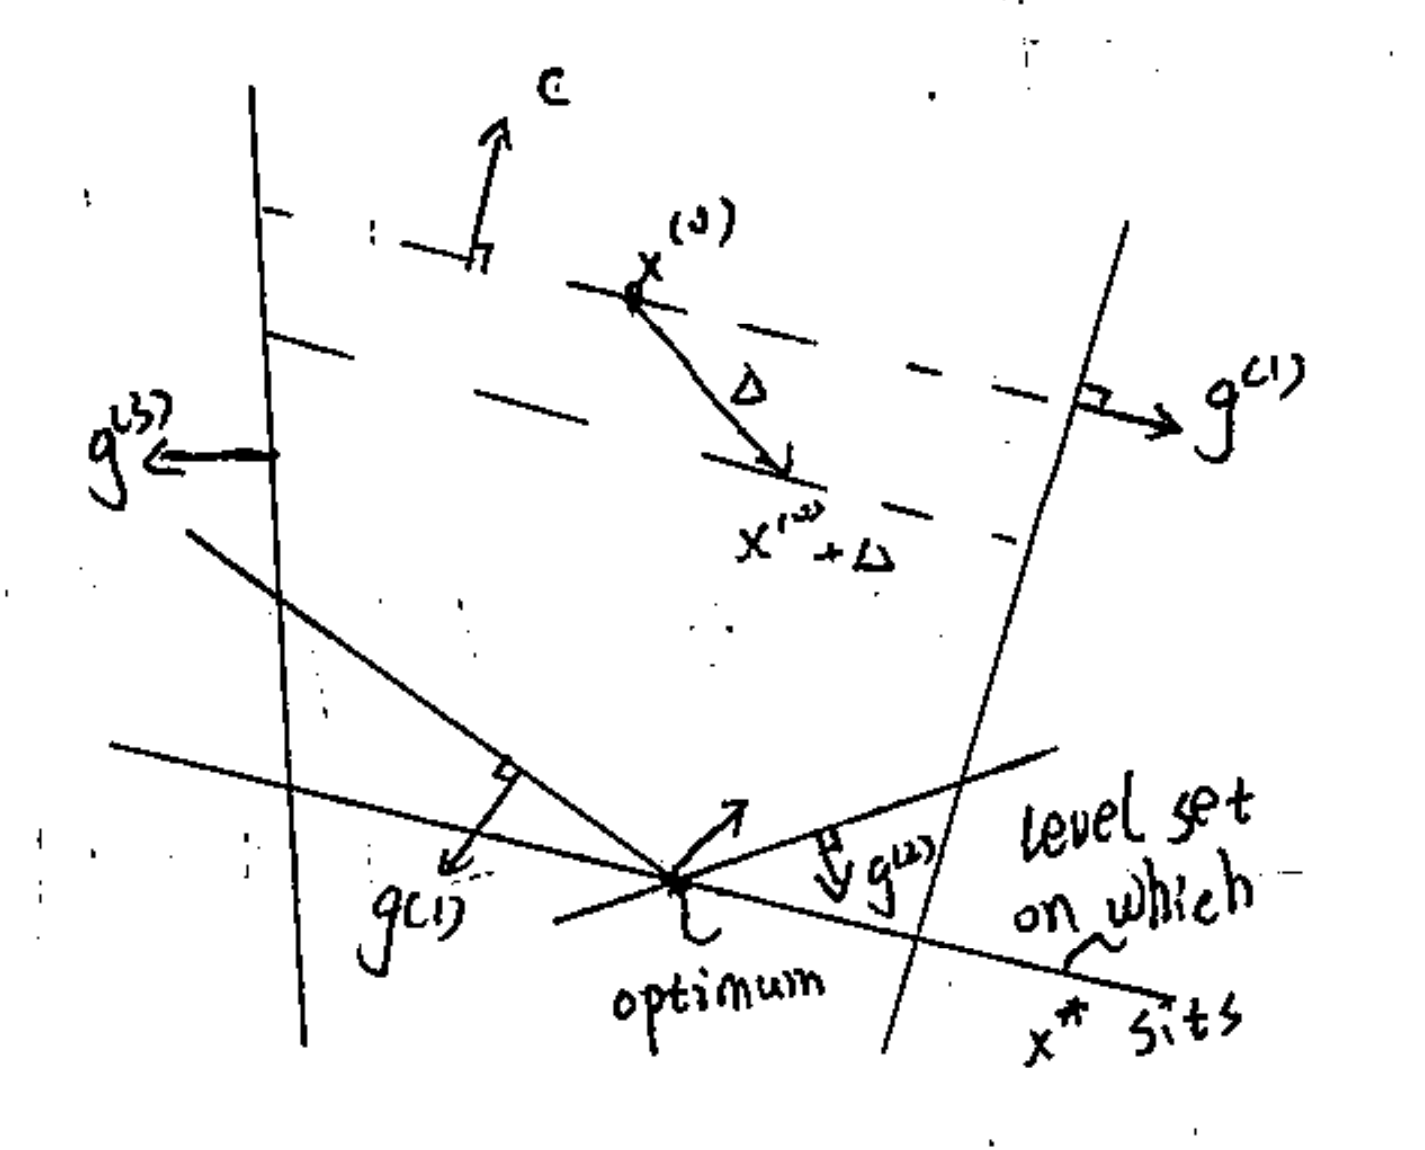
\includegraphics[width=2.1in,height=2.1in]{figures/ch07/figure1012_8.png}
		%\caption{This is an inserted JPG graphic} 
		%\label{fig:graph} 
	\end{figure}
	
	Active constraints: An optimal solution that lies at the intersection point of two constraints causes both of those constraints to be considered active
	
	Inactive constraints: If any of the constraint lines do not pass through the optimal point, those constraints are called inactive.
	
	In this example(see picture above) constraints g(1) and g(2) are active at optimum.
	
	Note that, we could improve(decrease) the cost if:
	$$c^{\trans}(x^{(0)} + \bigtriangleup) + d < c^{\trans}x^{(0)} + d$$
	That is, $\langle c, \bigtriangleup\rangle < 0$, the angle between displacement vector $\bigtriangleup$ and normal vector $c$ is an obtuse angle(see the picture above).
\end{example}





\vspace{0.5cm}
Some observations:
\begin{itemize}
	\item If you are at a vertex(doesn't have to be optimum). 
	
	\item Any "move" that keeps you feasible must also let you move into the feasible set 
	
	$\rightarrow$ opposite vector that define active constraints.
	
	\begin{equation*}
		v - \alpha g^{(1)} - \beta g^{(2)}, \quad \alpha, \beta \geq 0
	\end{equation*}
	
	\item Are these any choices of $\alpha, \beta$ that decrease the cost?
	\begin{align*}
		c^{\trans}(v - \alpha g^{(1)} - \beta g^{(2)}) + d &\leq c^{\trans}x + d\\
		-\alpha \langle c, g^{(1)}\rangle  - \beta \langle c, g^{(2)}\rangle &\leq 0
	\end{align*}
\end{itemize}

If:

1) $\langle c, g^{(1)}\rangle < 0$

2) $\langle c, g^{(2)}\rangle < 0$

no more into feasible set will decrease the cost.\\ 

\vspace{0.5cm}
Condition for optimality:

A feasible vertex $v$: $v\in\{x|Gx \leq h \}$ is an optimal solution to LP with cost $F_0(x) = c^{\trans}x + d$ if $c^{\trans}g^{(i)} < 0$, $\forall i\in$ active set.\\

\begin{figure}
	\centering
	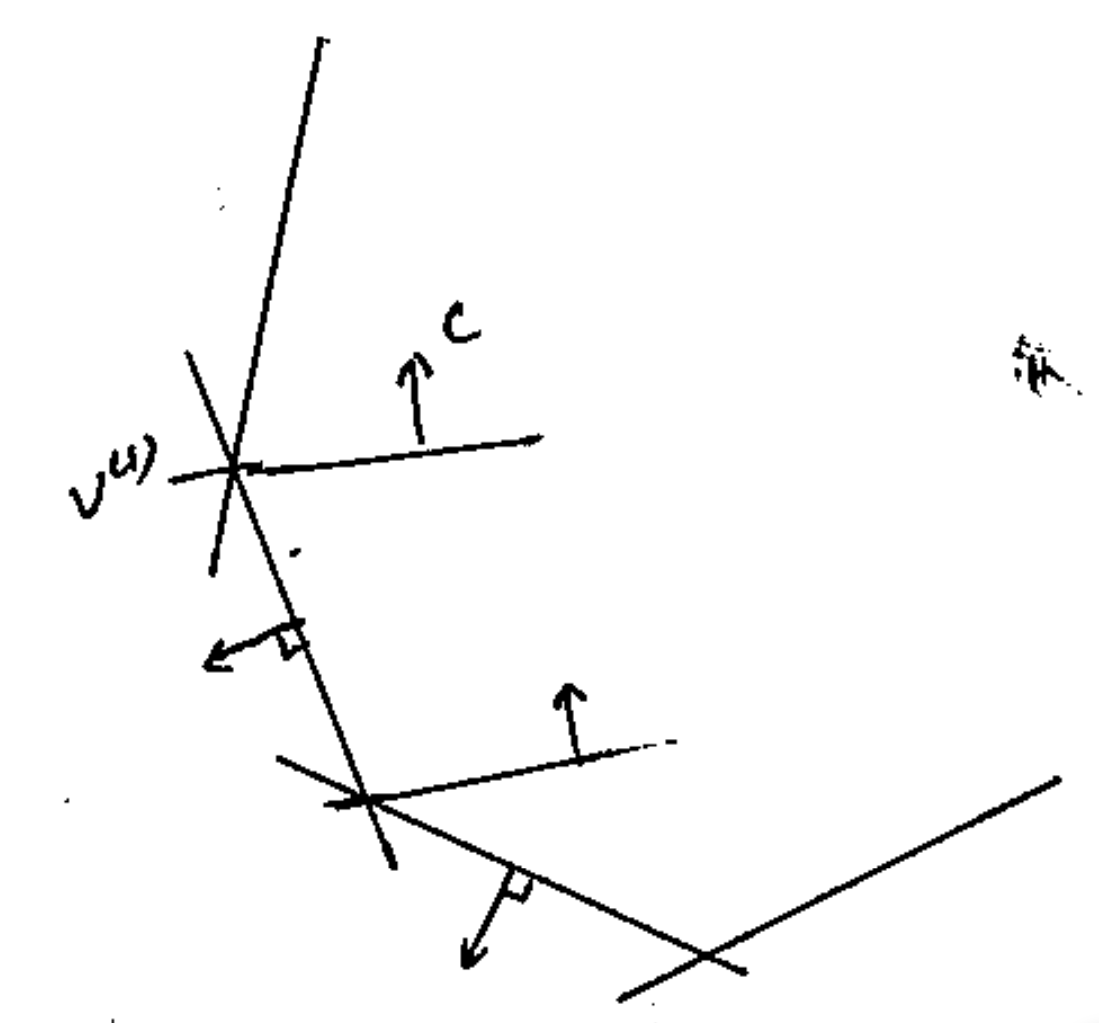
\includegraphics[width=2.1in,height=2.1in]{figures/ch07/figure1012_9.png}
	%\caption{This is an inserted JPG graphic} 
	%\label{fig:graph} 
\end{figure}


\subsection{Simplex Algorithm}
Simplex algorithm:
\begin{itemize}
	\item 1) Start from a feasible vertex;
	
	\item 2) Identify direction of cost decrease along an edge;
	
	\item 3) Move on that direction until any further more would violate a previously inactive constraints.
	
	\item 4) Stop + add that new constraint(s) to active set.
	
	\item 5) Repeat
\end{itemize}




%\begin{equation*}
%\{x|Gx\leq h \}
%\end{equation*}


%\begin{figure}
%	\centering
%	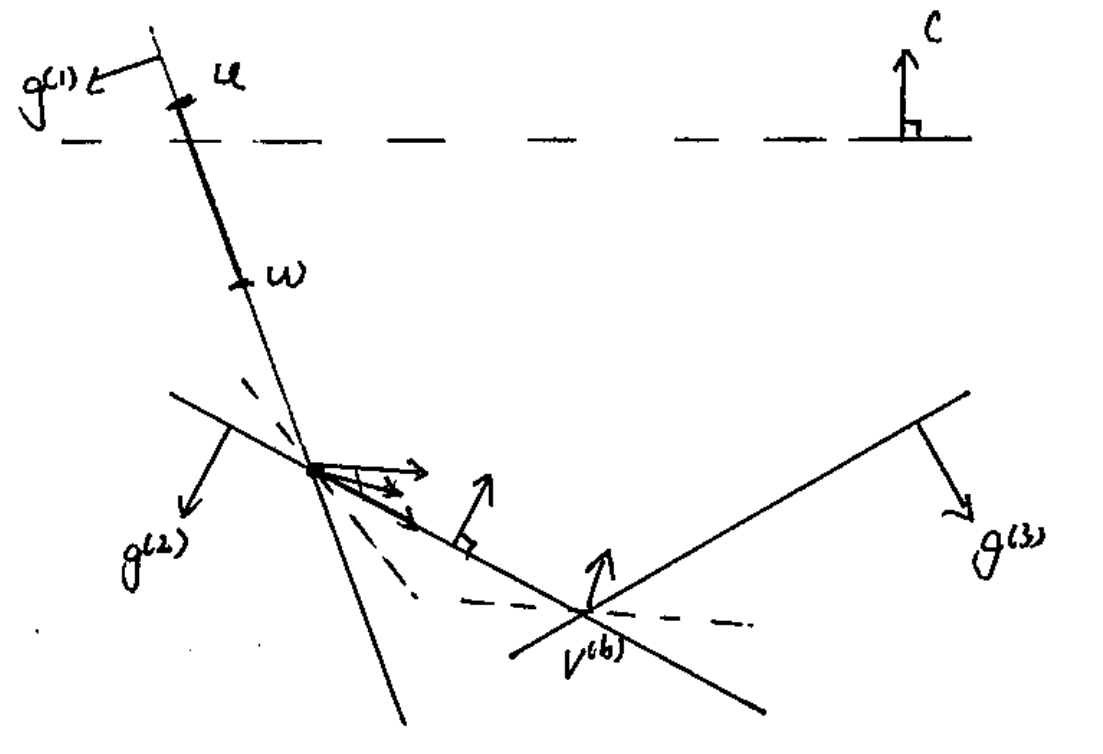
\includegraphics[width=2.1in,height=2.1in]{figures/ch07/figure1016_1.png}
%\caption{This is an inserted JPG graphic} 
%\label{fig:graph} 
%\end{figure}


%If $x =v^{(a)}$, constraints, constraints 1\&2 active, 3 is inactive.

%\begin{align*}
%<g^{(1)}, v^{(a)}> &= h_1\\
%<g^{(2)}, v^{(a)}> &= h_2\\
%<g^{(3)}, v^{(a)}> &< h_3
%\end{align*}

%At $x = v^{(b)}$, constraints 2\&3 active, 1 is inactive.\\

%1) Define a vertex $v$:

%\begin{itemize}
%	\item a) $v\in S$ is a vertex if cannot express $v = \lambda u +(1-\lambda)w$, $u, w\in S$, $\lambda \in [0,1]$

%	\item b) There exists a cost vector $c\in \reals^n$ s.t. $v$ is unique solution to an LP with cost vector $c$.

%	\item c) Algebraic characterization of vertices in terms of $A, b, G, h$. $S = \{x|Ax \leq b, Gx\leq h \}$
%\end{itemize}



%2) Define / Find directions along edges of polyhedron that keep you in the feasible set.

%3) How far can you go in direction that decrease cost until "leave" feasible set?


\begin{example}
	Consider the problem:
	\begin{align*}
		&min \Vert Ax - b\Vert_{\infty}\\
		&s.t. Gx \leq h
	\end{align*}
	
	Recall that $\Vert u\Vert_{\infty} = max_{i\in [n]}|u_i|$,
	\begin{figure}
		\centering
		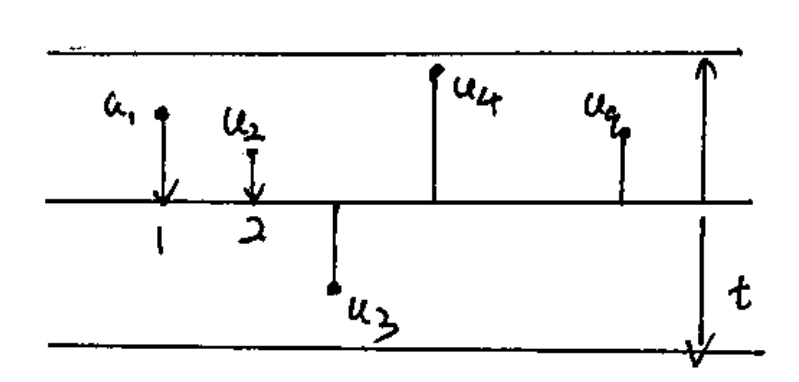
\includegraphics[width=2.1in,height=2.1in]{figures/ch07/figure1016_2.png}
		%\caption{This is an inserted JPG graphic} 
		%\label{fig:graph} 
	\end{figure}
	
	Introduce a helper(auxiliary) variable $t\in \reals$ which corresponding to the value of the norm, so the we convert the original problem into following problem:	
	\begin{align*}
		min &\qquad t\\
		s.t. &Ax - b\leq t\textbf{1}\\
		&Ax - b\geq (-t)\textbf{1}\\
		&Gx \leq h
	\end{align*}
\end{example}


\begin{example}
	Consider the problem:
	\begin{align*}
		\min_x &\Vert Ax - b\Vert _1, \qquad A\in \reals^{q\times n}\\
		s.t. &Gx\leq h
	\end{align*}
	\begin{figure}
		\centering
		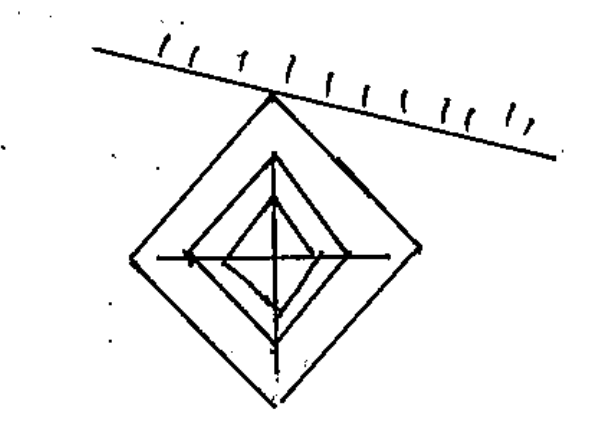
\includegraphics[width=2.1in,height=2.1in]{figures/ch07/figure1016_3.png}
		%\caption{This is an inserted JPG graphic} 
		%\label{fig:graph} 
	\end{figure}
	
	Recall the definition of $L_1$ norm:
	\begin{equation*}
		\Vert u\Vert_1 = \sum^q_{i=1} |u_i|
	\end{equation*}
	
	%	\begin{figure}
	%		\centering
	%		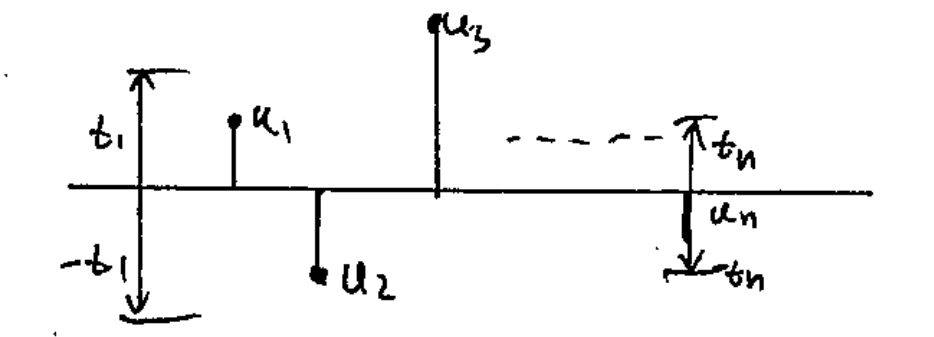
\includegraphics[width=2.1in,height=2.1in]{figures/ch07/figure1016_4.png}
	%		%\caption{This is an inserted JPG graphic} 
	%		%\label{fig:graph} 
	%	\end{figure}
	
	Let's introduce the helper vector $t\in \reals^q$,
	\begin{align*}
		\min_{x,t} &\sum^q_{i=1}t_i\\
		s.t. \quad&Gx \leq h\\
		&Ax -b \leq t\\
		&Ax -b \geq -t
	\end{align*}
	
\end{example}



\begin{example}
	Consider following problem:
	\begin{align*}
		min \quad max_{i\in [q]} &(c^{(i)^{\trans}}x + d_i)\\
		s.t. &Gx\leq h
	\end{align*}
	This case is similar to the $L_\infty$ norm case due to the inner max function, but it is one-sided(no lower bound). So we could convert the original one to the following:
	\begin{align*}
		min  &\qquad t\\
		s.t. &(c^{(i)^{\trans}}x + d_i)\leq t,\quad \forall i\in [q]\\
		&Gx\leq h
	\end{align*}
	\begin{marginfigure}
		\centering
		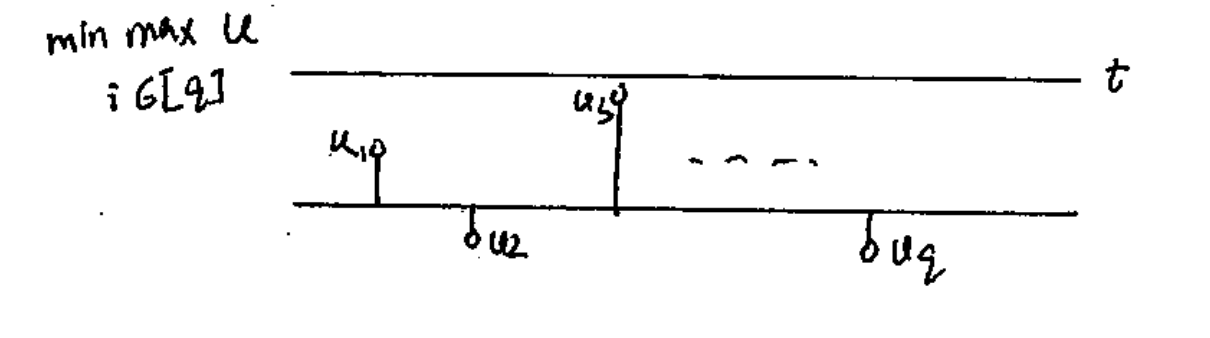
\includegraphics[width=2.1in,height=2.1in]{figures/ch07/figure1016_5.png}
		%\caption{This is an inserted JPG graphic} 
		%\label{fig:graph} 
	\end{marginfigure}
\end{example}

Remark:

In above three examples, the decision variables in initial formulation are $x\in \reals^n$, but in reformulation they become:

Example 7.6: $(x, t) \in \reals^n \times \reals$

Example 7.7: $(x, t) \in \reals^n \times \reals^n$

Example 7.8: $(x, t) \in \reals^n \times \reals$



\begin{example}
	Finding the largest $L_2$ ball that fits in a polytope.
	
	Let $p = \{x\in \reals^n| Gx\leq h \}$,
	
	\begin{figure}
		\centering
		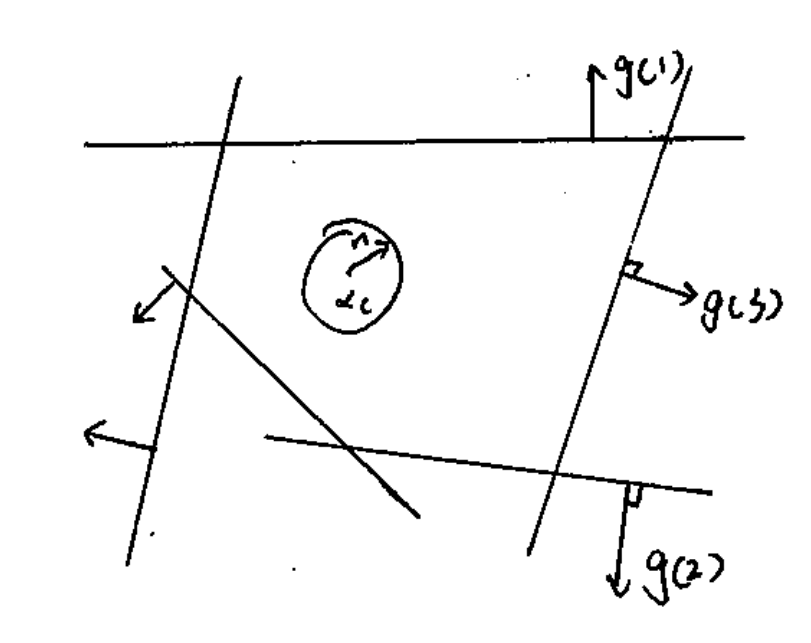
\includegraphics[width=2.1in,height=2.1in]{figures/ch07/figure1016_6.png}
		%\caption{This is an inserted JPG graphic} 
		%\label{fig:graph} 
	\end{figure}
\end{example}

It turns out that, this problem can be formulated as an LP problem. \

Note that:
\begin{itemize}
	\item A sphere is fully parameterized by its center $x_c$ and its radius $r$
	
	\item A sphere $(x_c, r)$ fits in $p$ if: $x_c + u \in p$, $\forall u \quad s.t. \Vert u\Vert _2\leq r$
\end{itemize}

\vspace{0.3cm}
Now, let's formulate as an LP. To accomplish this, observe that 

$x_c+u \in p$ means that $g^{(i)^{\trans}}(x_c + u) \leq h_i,\quad \forall i\in [q]$, $\forall u$ s.t. $\Vert u\Vert _2\leq r$.

\vspace{0.2cm}
Examine the constraint $g^{({i})^{\trans}}x_c + g^{({i})^{\trans}}u \leq h_i$ at a time:

As for $g^{({i})^{\trans}}u$, what's the direction of $u$ in order to make this term large as possible? It turns out, $u$ must be aligned with $g^{(i)}$, the same direction with $g^{(i)}$.

Furthermore, what's the value of $u$ that is aligned with $g^{(i)}$ and satisfies  $\vert u\vert_2=r?$ It should be:
$$u^*=\frac{g^{(1)}}{\Vert g^{(1)}\Vert }r$$


So, if the following is satisfied:
$$g^{(i)^{\trans}}[x_c + u^*] \leq h_i$$\
Then constraint $i$ will be satisfied for all $u$ such that $\vert u\vert \leq r$.

Substituting in $u^*$, the constraints become:
$$g^{(i)^{\trans}} x_c + \Vert g^{(i)}\Vert_2 r\leq h_i$$
Note that the constraint is linear in $x_c$ and $r$.

The problem of finding the largest sphere becomes the following:
\begin{align*}
	\max \quad & r\\
	s.t.\quad &g^{(i)^{\trans}}x_c + r \Vert g^{(i)}\Vert _2\leq h_i \qquad \forall i\in [q]
\end{align*}


Remarks:

(1) Optimal value $(x_c, r)\in \reals^{n+1}$.

(2) $x_c$ is a variable that does not enter the objective.

(3) Possibly no solution if $p$ is an empty set.

(4) Constraints and objective are linear in optimal variable so it is an LP problem.

(5)Transformed some quadratic-like problem (quadratic as a sphere is involved) into an LP, because we were able to identify which direction of $u$ the worst case for each constraint.






\newpage

\section{Quadratic program(QP)}

A quadratic programming problem is formulated in a general way as follows
\begin{align*}
p^* = \min_{x\in \reals^n}\quad &\frac{1}{2}x^{\trans}Hx + c^{\trans}x + d\\
 s.t.\quad &Ax = b\\
 &Gx\leq h
\end{align*}

The feasible set(feasible region) is illustrated as follows
\begin{figure}
	\centering
	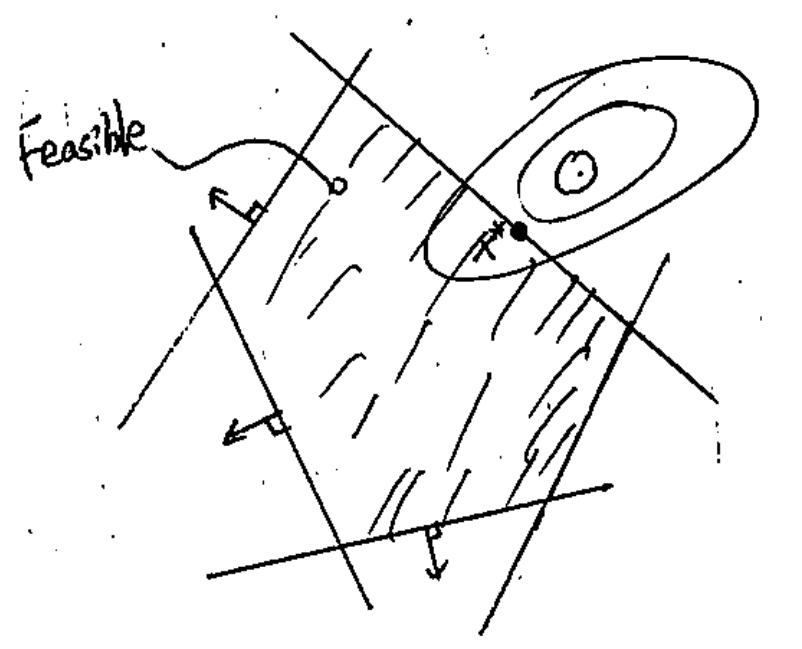
\includegraphics[width=2.1in,height=2.1in]{figures/ch07/figure1016_a.png}
	%\caption{This is an inserted JPG graphic} 
	%\label{fig:graph} 
\end{figure}

\subsection{Connection between LS problem and QP problem}
Recall the lest square problem we have studied, it turns out that we can convert the least square problem into a QP problem.
\begin{align*}
\Vert Ax - y\Vert _2^2 &= (Ax - y)^{\trans}(Ax - y)\\
&= x^{\trans}A^{\trans}Ax - 2y^{\trans}Ax + y^{\trans}y\\
&= \frac{1}{2}x^{\trans}(2A^{\trans}A)x - 2y^{\trans}Ax + \Vert y\Vert _2^2
\end{align*}

However, for the converse case, we can not always manipulate the objective of a QP into a  LS problem.


\subsection{Equality constrained QPs: Substitute back to the objective}
A basic idea of solving such kind of problem is to substitute the equality constraints back to the objective function so that hopefully we can eliminate some variables(dimensions), and obtain an unconstrained QP problem.

Consider a formulation of such kind of problem,
\begin{align*}
p^* = min_{x\in \reals^n}\quad &\frac{1}{2}x^{\trans}Hx + c^{\trans}x + d\\
s.t.\quad &Ax = b
\end{align*}


\begin{figure}
	\centering
	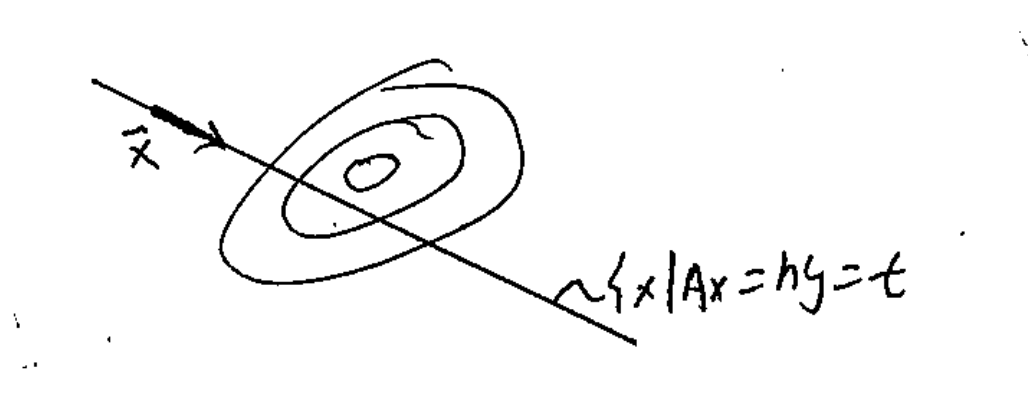
\includegraphics[width=2.1in,height=2.1in]{figures/ch07/figure1016_b.png}
	%\caption{This is an inserted JPG graphic} 
	%\label{fig:graph} 
\end{figure}

The feasible set could be expressed as follows
$$\mathcal{A} =\{x | x = \bar{x} + \xi,\quad \text{where } \xi \in N(A) \}$$
where $\bar{x}$ is a particular solution to the equation $Ax=b$.

Let $N$ be a basis for $N(A)$, so that we can express $\xi \in N(A)$ as $\xi = Nz$, where $z\in \reals^k$, $k =\text{dim}(N(A)) \leq n$.

Substitute this expression for any feasible $x$ into the objective $F_0(\cdot)$
\begin{align*}
F_0(x) 
&= F_0(\bar{x} + \xi)\\
&= F(\bar{x} + Nz)\\
&= \frac{1}{2}(\bar{x} + Nz)^{\trans}H(\bar{x}+Nz) + c^{\trans}(\bar{x} + Nz) + d\\
&= \frac{1}{2}z^{\trans}[N^{\trans}HN]z + [c^{\trans}N + \bar{x}^{\trans}HN]z + [\frac{1}{2}\bar{x}^{\trans}H\bar{x} + c^{\trans}x + d] \\
&= \frac{1}{2}z^{\trans}\tilde{H}z + \tilde{c^{\trans}}z + \tilde{d}\\
\end{align*}
where we newly define $\tilde{H}$, $\tilde{c^{\trans}}$, and $\tilde{d}$ in the last equality. So now we have obtain an unconstrained QP problem which is formulated as
\begin{equation*}
p^* = min_{z\in \reals^k}\quad \frac{1}{2}z^{\trans}\tilde{H}z + \tilde{c^{\trans}}z + \tilde{d}
\end{equation*}

Hence, to summarize,

(1)We have got a newly lower-dimensional optimization problem since $k =\text{dim}(N(A)) \leq n $.

(2)The new problem is still a QP, but is an unconstrained QP.



\begin{example}{Markowitz Portfolio optimization/Mean/variance" analysis}  Harry Markowitz(1990 Nobel Prize)
	
	
	\textbf{Problem formulation}: 
	\begin{itemize}
		\item Objective: For a fixed level of (expected) returns, we want to minimize the variance of returns.
		
		\item There are $n$ stocks, and we only consider a single investment period\\
		
		\item Design an optimal investment strategy $p\in \reals^n$, where the component $p_i = $ is the weight of your total wealth invested in the stock $i$.
		
		\item We require $\sum^n_{i=1}p_i = 1$, that is, you must invest all your money.
		
		\item We also require $p_i \geq 0$, that is, you are only allowed to take long positions, and short selling is not allowed.
		
		\item Your total wealth is normalized to $1$. So $p_i$ is not only weight but also the amount of money you invest on stock $i$ now.
	\end{itemize} 
	
	\textbf{Return and Variance}:
	
	\begin{itemize}
		\item Let $x\in \reals^n$ be a random vector denotes the return of $n$ stocks, so component $x_i$ is the return on the $i$-th stock in one period. That is, if we invest 1 RMB in a stock at the beginning, we will get $x_i$ RMB back at the end of this period.

		\item Expected returns: $\bar{x_i} = \mathbb{E}[x_i]$. In general, it is a known estimator based on historical data.
		
		\item Your return (random) is $\sum^n_{i=1}p_ix_i = p^{\trans}x$
		
		\item Your expected return $\mathbb{E}[\sum^n_{i=1}p_ix_i] = \sum^n_{i=1}p_i\mathbb{E}[x_i] = \sum^n_{i=1}p_i\bar{x_i} = p^{\trans}\bar{x}$
		
		\item variance in your return:
		\begin{align*}
		var(p^{\trans}x) &=\mathbb{E}[(p^{\trans}x - p^{\trans}\bar{x})^2]\\
		&= \mathbb{E}[(p^{\trans}(x - x^{\trans}))^2]\\
		&= \mathbb{E}[p^{\trans}(x - \bar{x})(x - \bar{x})^{\trans}p]\\
		&= p^{\trans}\mathbb{E}[(x - \bar{x})(x - \bar{x})^{\trans}]p\\
		&= p^{\trans}\Sigma p
		\end{align*}
	\end{itemize}
	
	
	With above terminology and model formulation, given a mean return $\bar{x}$ and the covariance matrix of returns $\Sigma \in \reals^{n\times n}$, we want to find an optimal strategy/policy $p$ to minimize the risk(represent by variance) subject to same minimal returns.: 
	
	The problem is formulated as:
	\begin{align*}
	min_{p\in \reals^n}\quad &p^{\trans}\Sigma p\\
	s.t. \quad&p^{\trans}\bar{x}\geq r_{min}\\
	&\textbf{1}^{\trans}p = 1\\
	&p\geq 0
	\end{align*}
\end{example}



\subsection{Geometry of QP}
Consider the general form of QP
\begin{align*}
p^* = min_{x\in \reals^n}\quad &\frac{1}{2}x^{\trans}Hx + x^{\trans}x + d\\
s.t.\quad &Ax = b\\
&Gx\leq h
\end{align*}
Follow the same as LP, we would like to discuss the geometry of QP.

\begin{marginfigure}
	\centering
	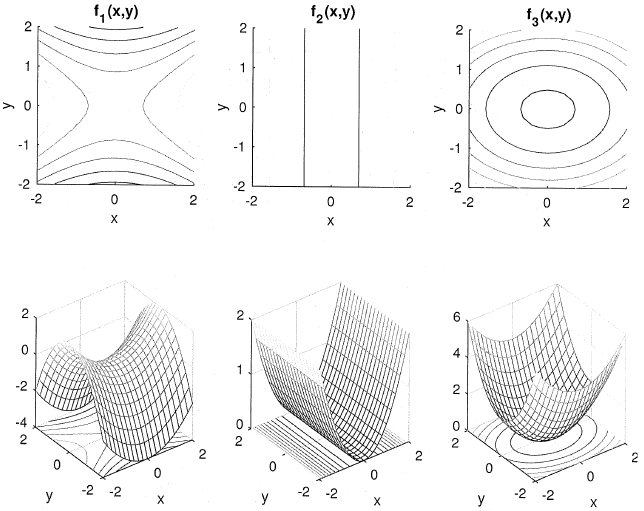
\includegraphics[width=2.5in,height=3in]{figures/ch07/figure1112_01.png}
	\caption{Plot 1} 
	%\label{fig:graph} 
\end{marginfigure}


\begin{marginfigure}
	\centering
	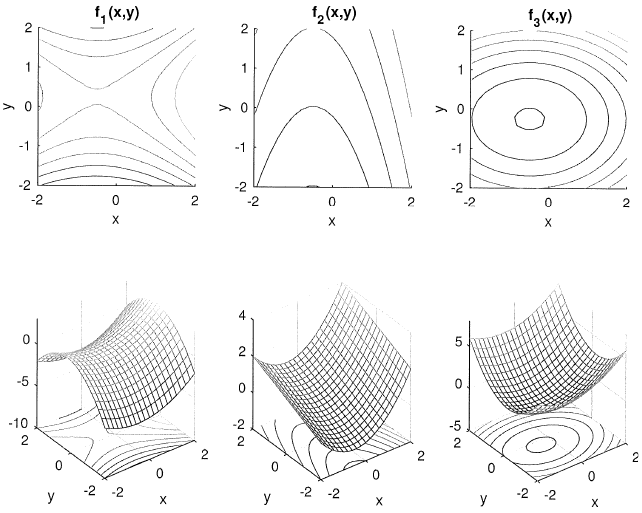
\includegraphics[width=2.5in,height=3in]{figures/ch07/figure1112_02.png}
	\caption{Plot 2} 
	%\label{fig:graph} 
\end{marginfigure}


\begin{marginfigure}
	\centering
	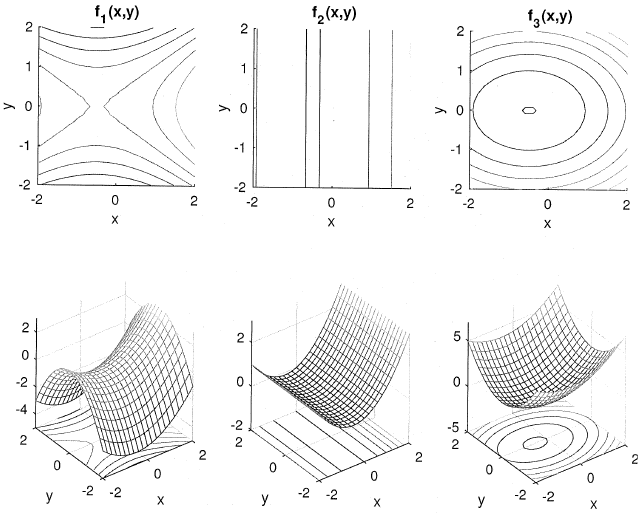
\includegraphics[width=2.5in,height=3in]{figures/ch07/figure1112_03.png}
	\caption{Plot 3} 
	%\label{fig:graph} 
\end{marginfigure}

(1) Geometry of feasible set: The same as LP.

(2) Geometry of objective: Without loss of generality(w.l.o.g), we can assume that $H\in S^n$, i.e., $H$ is symmetric, since
\begin{align*}
x^{\trans}Hx 
&=\frac{1}{2}[x^{\trans}Hx + x^{\trans}H^{\trans}x]\\
&= \frac{1}{2}x^{\trans}(H+H^{\trans})x
\end{align*}
clearly $H$ is symmetric.\\

Recal that for symmetric matrices, we have

a) Eigenvalues: purely real eigenvalues (so we can arrange them in an order).

b) Eigenvectors: can be chosen to be $\perp$ and can always diagonalize $H$, i.e., we can write
$$H = \mathcal{U}\Lambda \mathbb{U}^{\trans}  = \sum^n_{i=1}\lambda_iu^{(i)}u^{(i)^{\trans}}$$

Consider following 3 different cases for the matrix $H$:
\begin{itemize}
	\item A) $H\in S^n$ but not PSD
	
	\begin{equation*}
	H = 
	\begin{bmatrix}
	1&0\\
	0&-2
	\end{bmatrix}
	\end{equation*}
	
	\item B) $H\in S^n_+$ but not PD
	\begin{equation*}
	H = 
	\begin{bmatrix}
	1&0\\
	0&0
	\end{bmatrix}
	\end{equation*}
	
	\item C) $H\in S^n_{++}$
	\begin{equation*}
	H = \begin{bmatrix}
	1&0\\
	0&2
	\end{bmatrix}
	\end{equation*}
\end{itemize}

%Now, let's look at visualization for cases A to C.

%If we only consider the quadratic term,
%$$F_0(x) =\frac{1}{2}x^{\trans}Hx$$
%Clearly, we have following results

Consider the 3 cases for $H$ given above and the following different objective functions, we plot these figures on r.h.s. for illustration.

Plot 1: $F_0(x) =\frac{1}{2}x^{\trans}Hx$

Plot 2: $F_0(x) =\frac{1}{2}x^{\trans}Hx + [0.5\quad 0.5]x$

Plot 3: $F_0(x) =\frac{1}{2}x^{\trans}Hx + [0.5\quad 0]x$


\vspace{0.5cm}
\textbf{Let's consider 3 different cases for a general QP problem.}

\textbf{Case A: } $H\in S^n$ but $H\notin S^n_+$ (Symmetric not PSD).

For such $H$, there must be an eigenvalue/vector pair $(\lambda, u)$ s.t. $\lambda < 0$.

Set $x_{\alpha} = \alpha u$ for some $\alpha \in \reals$, we have

\begin{align*}
F_0(\alpha u) &= \frac{1}{2}(\alpha u)^{\trans}H(\alpha u) + c^{\trans}(\alpha u) + d\\
&= \frac{{\alpha}^2}{2} u^{\trans}[\sum^n_{i=1}\lambda_i u^{(i)} u^{(i)^{\trans}}]u + \alpha c^{\trans}u + d\\
&= \frac{{\alpha}^2}{2}\lambda + \alpha <c,u> + d
\end{align*}

Since $\lambda<0$, let $\alpha \to \infty$ leads to an unbounded objective function, i.e., $p^* = -\infty$.



\vspace{0.3cm}
\textbf{Case B: } $H\in S_+^n$ but $H\notin S^n_{++}$ ($H$ is PSD but not PD)

$\rightarrow$ $H$ has at least 1 zero eigenvalue.\\

\vspace{0.3cm}
\textbf{Case B (i)} $H\in S_+^n$ but $H\notin S^n_{++}$ and $c \notin R(H)$.

There is a complement of $c$ in $R(H)^{\perp} = N(H^{\trans}) = N(H)$, and thus we can move in that direction without affecting $2^{nd}$ order term while driving $1^{st} $ order term to $-\infty$.

Let $c_{\Vert} = \prod_{R(H)}(c)$,  and $c_{\perp} = \prod_{N(H)}(c)$, where the first one is the component in $R(A)$ and second one is the component in $N(H)$.

Notice that $R(H)^{\perp}= N(H^{\trans}) = N(H)$, since $H$ is symmetric. By orthogonal decomposition lemma, there is an unique decomposition
$$c = c_{\Vert} + c_{\perp}$$

Now, let $x_{\alpha} =-\alpha c_{\perp}$, where $\alpha \in \reals_+$.
\begin{align*}
F_0(x_{\alpha}) 
&=\frac{{\alpha}^2}{2}c_{\perp}^{\trans}Hc_{\perp} + c^{\trans}(-\alpha c_{\perp}) + d\\
&= 0 - \alpha(c_{\Vert} + c_{\perp})^{\trans}c_{\perp} + d\\
&= -\alpha(c_{\Vert}^{\trans}c_{\perp} + c_{\perp}^{\trans}c_{\perp}) + d\\
&= -\alpha \Vert c_{\perp}\Vert^2_2 + d
\end{align*}

Hence the function is unbounded below since we could take $\alpha \to\infty$. Therefore,
$$p^*=-\infty$$



\vspace{0.3cm}
\textbf{Case B (ii)}  $H\in S_+^n$ but $H\notin S^n_{++}$ and $c \in R(H)$.

First, remind us of some results from previous chapter,
\begin{align*}
H 
&= \sum^n_{i=1}\lambda_i U^{(i)}U^{(i)^{\trans}} \\
&= \sum^r_{i=1}\lambda_i U^{(i)}U^{(i)^{\trans}}\\
&= U_r\Sigma Y_r^{\trans}
\end{align*}
and,
\begin{align*}
H^{\frac{1}{2}} &= U_r\Sigma^{\frac{1}{2}}U_r^{\trans}\\
H^{+} &= U_r\Sigma^{-1}U_r^{\trans}\\
(H^{\frac{1}{2}})^+ &= U_r\Sigma^{-\frac{1}{2}}U_r^{\trans}
\end{align*}

where 
$$\Sigma = 
\begin{bmatrix}
\sqrt{\lambda_1} &  & 0 \\
&\ddots&\\
0&&\sqrt{\lambda_r}
\end{bmatrix}
,\
\Sigma^{-\frac{1}{2}} =
\begin{bmatrix}
\frac{1}{\sqrt{\lambda_1}} &  & 0 \\
&\ddots&\\
0&&\frac{1}{\sqrt{\lambda_r}}
\end{bmatrix}
$$

Observe that
$$C\in R(H) = R(H^{\frac{1}{2}}) = R(H^+) = R\left((H^{\frac{1}{2}})^+\right)$$

Since $C\in R(H)$ and $R(H) = R(H^{\frac{1}{2}})$, there exists $y \in \reals^n$ such that
$$C = H^{\frac{1}{2}}y = H^{\frac{1}{2}}(y+\xi)$$

where $\xi \in N(H^{\frac{1}{2}})$. Note that choice of $y$ is not unique and the second equality due to $\rank(H)= r<n$. 

Explicitly, we have 
\begin{equation*}
C = (U_r\Sigma^{\frac{1}{2}}U_r^{\trans})y = \sum^r_{i=1}U^{(i)}\sqrt{\lambda_i}(U^{(i)^{\trans}}y)
\end{equation*}

Now, the question is, which $y$ we should pick? Let's pick the $y$ with min-norm, that is, 
\begin{align*}
y &=\arg\min_{\bar{y}\in\reals^n}\Vert \bar{y}\Vert_2\\
s.t\  C &= H^{\frac{1}{2}}\bar{y}
\end{align*}

It turns out that, this is an under determined and rank-deficient LS problem. So the solution to this question is given by
$$y = (H^{\frac{1}{2}})^+C = U_r \Sigma^{-\frac{1}{2}} U_r^{\trans} C$$


So, when $C = H^{\frac{1}{2}}y$, we can pick $y = (H^{\frac{1}{2}})^+C$. Let's look back at the objective to understanding such choice.
\begin{align*}
\frac{1}{2}x^{\trans}Hx + c^{\trans}x + d &= \frac{1}{2}x^{\trans}H^{\frac{1}{2}}H^{\frac{1}{2}}x+y^{\trans}H^{\frac{1}{2}}x + d\\
&= \frac{1}{2}\tilde{x}^{\trans}\tilde{x} + y^{\trans}\tilde{x} + d\\
&= \frac{1}{2}(\tilde{x}^{\trans}x+2y^{\trans}\tilde{x}+y^{\trans}y) - \frac{1}{2}y^{\trans}y + d \\
&= \frac{1}{2}\Vert\tilde{x}+y\Vert^2_2 - \frac{1}{2}\Vert y \Vert^2_2 + d &(*)
\end{align*}
In the second equality we let $\tilde{x} = H^{\frac{1}{2}} x$.

Apparently, we would like to set $\tilde{x} = -y$ to minimize $(*)$, and the question is, is this always possible? The answer is yes.

Since $y = (H^{\frac{1}{2}})^+C\in R((H^{\frac{1}{2}})^+) = R(H) = R(H^{\frac{1}{2}})$, and $\tilde{x}=H^{\frac{1}{}} x$ so $\tilde{x} \in R\left(H^{\frac{1}{2}}\right) = R(H)$. Since $x\in \reals^n$ is unconstrained, so we can choose $x$ to make $\tilde{x}$ equal to any element of $R(H)$, namely $y$. 

Thus, to minimize $(*)$ we set $\tilde{x} = -y$ where $\tilde{x} = H^{\frac{1}{2}}x$, and yields
\begin{align*}
F_0(x) \geq p^* &= d - \frac{1}{2}\Vert y \Vert_2^2\\
&= d - \frac{1}{2}y^{\trans}y\\
&= d - \frac{1}{2}C^{\trans}(H^{\frac{1}{2}})^+(H^{\frac{1}{2}})^+C\\
&= d - \frac{1}{2}C^{\trans}
\begin{bmatrix}
U_r
\end{bmatrix}
\begin{bmatrix}
\Sigma^{-\frac{1}{2}}]
\end{bmatrix}
\begin{bmatrix}
U_r^{\trans}
\end{bmatrix}
\begin{bmatrix}
U_r
\end{bmatrix}
\begin{bmatrix}
\Sigma^{-\frac{1}{2}}]
\end{bmatrix}
\begin{bmatrix}
U_r^{\trans}
\end{bmatrix}
\begin{bmatrix}
C
\end{bmatrix}\\
&= d - \frac{1}{2}C^{\trans}(U_r\Sigma^{-1}U^{\trans}_r)C\\
&= d - \frac{1}{2}C^{\trans}H^+C
\end{align*}

What is the minimizing choice of $x\in \reals^n$?

Since $y\in R(H) = R(H^{\frac{1}{2}})$ and $x\in \reals^n$ is free, we can satisfy equality and thus there are many solutions. 

We would like to pick min-norm solution for $x$, which is given by
\begin{align*}
x^* 
&= (H^{\frac{1}{2}})^+\tilde{x}\\
&= -(H^{\frac{1}{2}})^+y\\
&= -(H^{\frac{1}{2}})^+(H^{\frac{1}{2}})^+C\\
&= -H^+C
\end{align*}\\

\vspace{0.3cm}
\textbf{Case C}: $H\in S^n_{++}$ ($H$ is PD)

This is indeed a special case of case B(ii), and that's because

(1)$H\in S^n_{++}$, then it is also in $S^n_{+}$, and so all eigenvalues are non negative.

(2)$H\in S^n_{++}$, then $\rank(H) = n$ and thus $R(H)=\reals^n$, and certainly $C \in R(H)$.

From previous solution, we have
\begin{align*}
x 
&= -H^{+}C\\
&= -U_r \Sigma^{-1} U_r^{\trans} C\\
&= -U_r \Sigma^{-1} U_n^{\trans} C\\
&= - H^{-1} C
\end{align*}
So in this case $H^+ = H^{-1}$. The optimal value is given by
$$p^* = d - \frac{1}{2}C^{\trans}H^{-1}C$$


\textbf{Summary }

Consider the QP problem $p^* = min_{x\in \reals^n}\frac{1}{2}x^{\trans}Hx + c^{\trans}x + d$,
\begin{equation}
p^* = \left\{
\begin{array}{lr}
d - \frac{1}{2}c^{\trans}H^+c &\text{$H$ is PD, or, $H$ is PSD but not PD and $c \in R(H)$}\\
-\infty &\text{$H$ is not PSD, or, $H$ is PSD but not PD and $c\notin R(H)$}
\end{array}
\right.\nonumber
\end{equation}

\begin{equation}
x^* = \left\{
\begin{array}{lr}
-H^+c &\text{$H$ is PD, or, $H$ is PSD but not PD and $c \in R(H)$}\\
\text{not exist} &\text{$H$ is not PSD, or, $H$ is PSD but not PD and $c\notin R(H)$}
\end{array}
\right.\nonumber
\end{equation}

\vspace{0.5cm}
\subsection{Solving QPs via "active set" methods}

\begin{align*}
\min_{x\in \reals^2} \quad & (x_1 - 1)^2 + (x_2 - 2.5)^2 \\
s.t. \quad&
\begin{bmatrix}
-1&2\\
1&2\\
1&-2\\
-1&0\\
0&-1
\end{bmatrix}
\begin{bmatrix}
x_1\\
x_2
\end{bmatrix}
\leq
\begin{bmatrix}
2\\
6\\
2\\
0\\
0
\end{bmatrix}
\end{align*}

\begin{marginfigure}
	\centering
	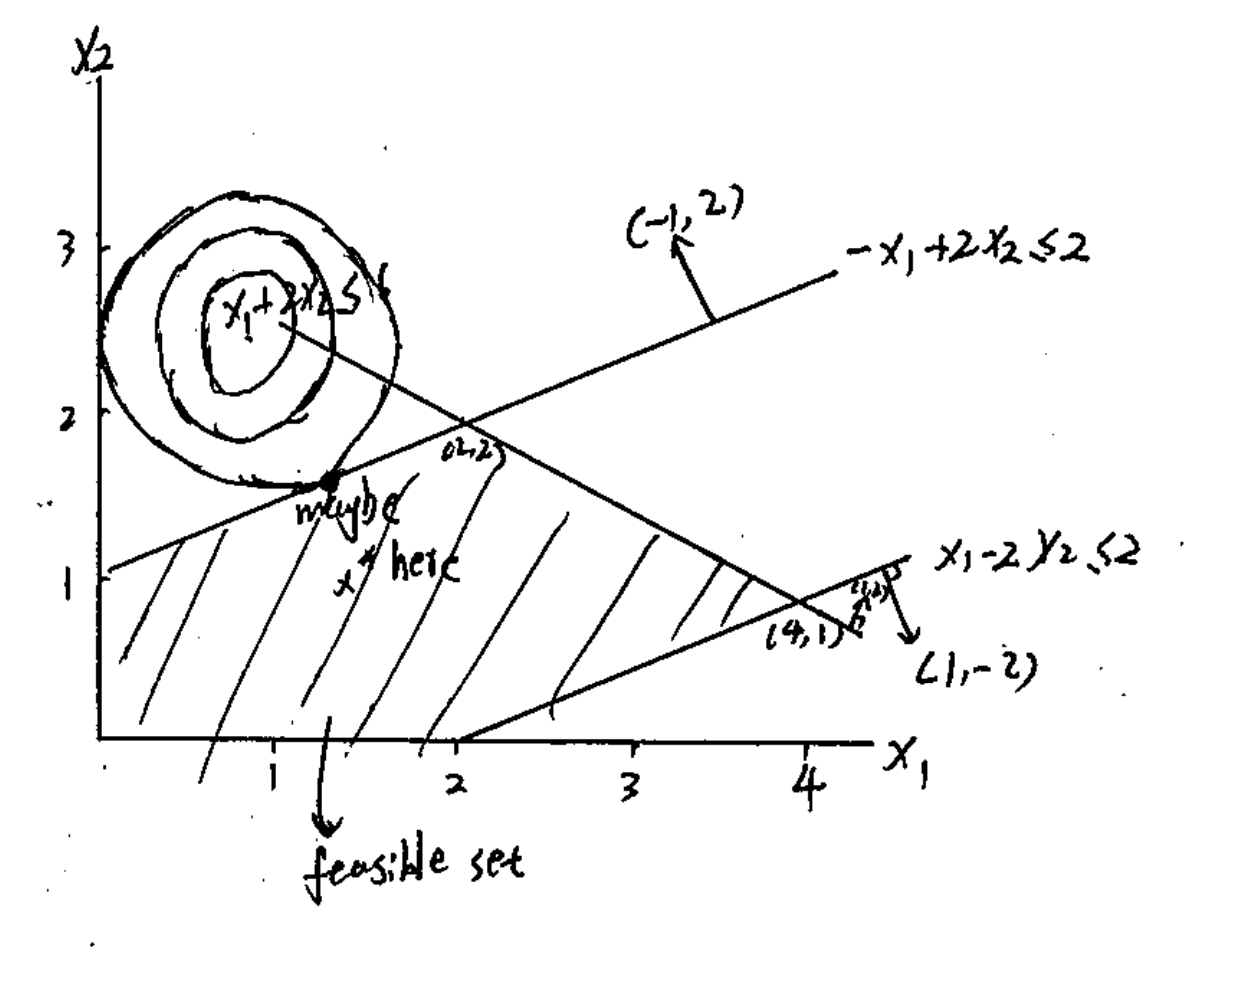
\includegraphics[width=1.8in,height=1.8in]{figures/ch07/figure1021_1.png}
	%\caption{This is an inserted JPG graphic} 
	%\label{fig:graph} 
\end{marginfigure}

\begin{itemize}
	\item at optimum some subset of inequality constraints satisfied with equality "active" set
	
	\item Best "loose"
	
	\item If you know the active set or optimum, just solve an "equality"-constrained QP"
\end{itemize}
By illustrative example:

Step 1

Initialize at point $x^{(0)} = \begin{bmatrix}
2\\
0
\end{bmatrix}$, starting with initial "working set" of equality constraint(the fifth equality constraint):
$$w_0 = \{x|x_2 = 0 \}$$


Step 2
 \begin{align*}
\min_{x\in \reals^2} \quad
&
\frac{1}{2}x^{\trans}
\begin{bmatrix}
2&0\\
0&2
\end{bmatrix}
x + 
\begin{bmatrix}
-2 & -5
\end{bmatrix} 
+ (1 + 2.5^2)\\
s.t.\quad &
\begin{bmatrix}
0 & 1
\end{bmatrix}
x = 0
\end{align*}


Recall the linearly constrained QP problem, we need a basis for 
$N(\begin{bmatrix} 
0\\
1
\end{bmatrix}) 
= \{x|x = \alpha
\begin{bmatrix}
1\\
0
\end{bmatrix} \}$
in this case. Let
$N=
\begin{bmatrix}
1\\
0
\end{bmatrix}$,

$$\tilde{H} = N^{\trans}HN = 2$$
$$\tilde{C}^{\trans} = (c^{\trans}N + \bar{x}^{\trans} HN)= -2$$
$$\tilde{d}= (d+c^{\trans}x + \frac{1}{2}\bar{x}^{\trans}H\bar{x})=0$$


So we have converted the problem to :
\begin{align*}
z^* 
&= \arg\min_{z\in\reals} \frac{1}{2} z^{\trans}\tilde{H}z + \tilde{c}^{\trans}z + \tilde{d}\\
&= \arg\min_{z\in\reals} \frac{1}{2}2z^2 + (-2z)+ 0\\
&= \arg\min_{z\in\reals} z^2 - 2z
\end{align*}
Take the first derivative and set it to zero, we get $z^* = 1$.

So the optimum is:
\begin{equation*}
x^{(1)}= \bar{x}+ z^*N = 
\begin{bmatrix}
0\\
0
\end{bmatrix}
 + 1
\begin{bmatrix}
1\\
0
\end{bmatrix} = 
\begin{bmatrix}
1\\
0
\end{bmatrix}
\end{equation*}


Step 3

Note:

(1) At this point we recognize that the equality constraint $\{x|x_2=0\}$ is no longer "binding" because we just optimized along that set.

(2) We could drop the fifth constraint from "working set" left with $w_2 =\emptyset$

(3) We are facing with an unconstrained optimization problem. Clearly we would like to move to $x^{(1)} +\Delta = 
\begin{bmatrix}
1\\
0
\end{bmatrix}
+
\begin{bmatrix}
0\\
2.5
\end{bmatrix}
$.

(4) But there may be a "blocking" constraint in way. In this example, this is the first constraint $\{x|-x_1 +2x_2\leq 2 \}$

(5) Instead, we solve for the a step size $\gamma$ to make the constraint light, i.e., $g^{(i)T}(x^{(1)}+\gamma \Delta) = h_1$. 

So we have,
$$[-1\ 2] 
\begin{bmatrix}
1\\
0
\end{bmatrix}
+
\gamma
\begin{bmatrix}
0\\
2.5
\end{bmatrix}
=
2
\Leftrightarrow
\gamma= \frac{3}{5}
$$

$$
x^{(2)} = x^{(1)} +\frac{3}{5} \Delta =
\begin{bmatrix}
1\\
1.5
\end{bmatrix}
$$


Step 4

This time, $w_3 = \{x|
\begin{bmatrix}
-1& 2
\end{bmatrix}
\begin{bmatrix}
x_1\\
x_2
\end{bmatrix}
=2
\}$.

$$N(
\begin{bmatrix}
-1& 2
\end{bmatrix})
=
\{x|x=\alpha
\begin{bmatrix}
2\\
1
\end{bmatrix}\},
\quad
\bar{x}\in 
\{x|
\begin{bmatrix}
-1& 2
\end{bmatrix}
\begin{bmatrix}
x_1\\
x_2
\end{bmatrix}
=2
\}
$$

We pick $N=
\begin{bmatrix}
2\\
1
\end{bmatrix}
,\quad
\bar{x}=
\begin{bmatrix}
0\\
1
\end{bmatrix}
$.

$$\tilde{H} = N^{\trans}HN = 10$$
$$\tilde{C}^{\trans} = (c^{\trans}N + \bar{x}^{\trans} HN)= -7$$
$$\tilde{d}= (d+c^{\trans}x + \frac{1}{2}\bar{x}^{\trans}H\bar{x})=-4$$

\begin{align*}
z^* 
&= \arg\min_{z\in\reals} \frac{1}{2} z^{\trans}\tilde{H}z + \tilde{c}^{\trans}z + \tilde{d}\\
&= \arg\min_{z\in\reals} \frac{1}{2}10 z^2 + (-7z) - 4\\
&= \arg\min_{z\in\reals} 5z^2 - 7z -4
\end{align*}
Take the first derivative and set it to zero, we get $z^* = \frac{7}{10}$.

\begin{equation*}
x^{(3)}= \bar{x}+ z^*N = 
\begin{bmatrix}
0\\
1
\end{bmatrix}
+ 
\frac{7}{10}
\begin{bmatrix}
2\\
1
\end{bmatrix} = 
\begin{bmatrix}
1.4\\
1.7
\end{bmatrix}
\end{equation*}

Note $x^{(3)}$ is the global optimum so we end this algorithm here.



\vspace{0.5cm}
\subsection{Quadratically Constrained Quadratic Program (QCQP)}
Let's formulate such kind of problem first
\begin{align*}
\min_{x\in \reals^n} \quad &\frac{1}{2}x^{\trans}H_0 x + c_0^{\trans} x + d_0\\
s.t.\quad &\frac{1}{2}x^{\trans}H_ix + c^{\trans}_i x + d_i \leq 0  & i\in [m]\\
&\frac{1}{2} x^{\trans} \tilde{H}_ix + \tilde{c}_i^{\trans}x + \tilde{d}_i = 0 & i\in [q]
\end{align*}

\textbf{Note:}

\begin{itemize}
	\item If $H_i = 0, \forall i\in [n]$, $\tilde{H}_i = 0, \forall i\in [q]$, then we have a $QP$.
	
	\item Typically $H_0\geq 0$, $H_i\geq 0$, $i\in [m]$, and $\tilde{H}_i = 0$, $\forall i\in [q]$, in which case the problem is a convex optimization problem, and thus it is easy to solve as we will discuss in next chapter.
	
\end{itemize}

To see that why $\tilde{H}_i \neq 0$ makes things difficult, let's consider a single  equality constraint $q = 1$, and a scalar problem $x\in \reals$:
$$\tilde{H}_1 = 1 \quad \tilde{c}_i = 0 \quad \tilde{d}_i = -\frac{1}{2}$$
So the equality constraint becomes:
$$\frac{1}{2}x_1^2 + 0 - \frac{1}{2} = 0 \Leftrightarrow x_1^2 = 1 \Leftrightarrow x_1\in\{-1, 1\} $$
Notice that the feasible set is not a continuum of possibilities, i.e., it is a distinct set so the problem is "Combinatorial".





\begin{example}
Let's consider the QCQP with only three inequality constraints ($m=3$).
\begin{marginfigure}
	\centering
	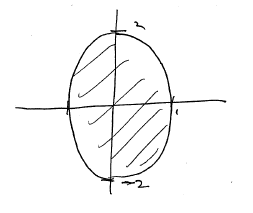
\includegraphics[width=1.8in,height=1.8in]{figures/ch07/figure1021_2.png}
	\caption{Feasible set of constraint 1} 
	%\label{fig:graph} 
\end{marginfigure}

Constraint 1:

\begin{equation*}
H_1=\begin{bmatrix}
2 & 0 \\
0 &\frac{1}{2}
\end{bmatrix}
\qquad 
c_1^{\trans} = \begin{bmatrix}
0 & 0
\end{bmatrix}
\qquad 
d_1 = -1
\end{equation*}

So this constraint can be written as
\begin{align*}
\frac{1}{2}x^{\trans}H_1x + c_1^{\trans}x + d_1 \leq 0 &\Leftrightarrow 2x_1^2 + \frac{1}{2}x_2^2 \leq 2\\
&\Leftrightarrow\frac{x_1^2}{1} + \frac{x_2^2}{4}\leq 1
\end{align*}

It is obviously the feasible set of this constraint corresponds to an ellipse, and by computing the eigenvalues(lengths of major and minor axis) and eigenvectors(directions of major and minor axis) of $H_1$, we are able to draw such feasible set as on the r.h.s.

\begin{marginfigure}
	\centering
	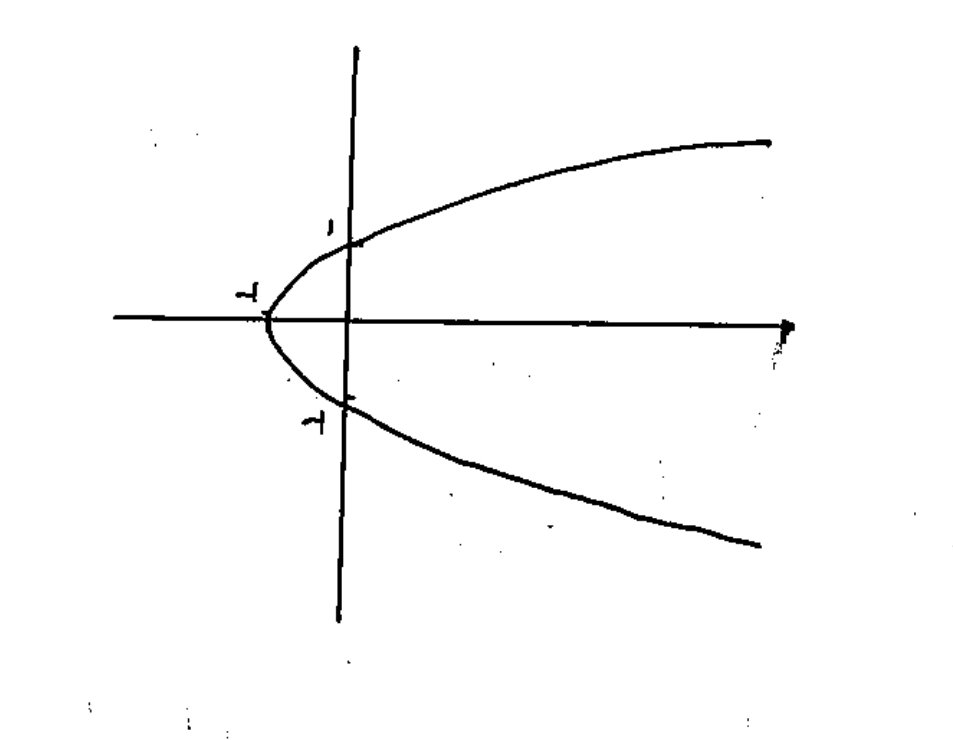
\includegraphics[width=1.8in,height=1.8in]{figures/ch07/figure1021_3.png}
	\caption{Feasible set of constraint 2} 
	%\label{fig:graph} 
\end{marginfigure}

Constraint 2:
\begin{equation*}
H_2=
\begin{bmatrix}
0 & 0\\
0 & 0
\end{bmatrix}
\qquad
c_2^{\trans} = 
\begin{bmatrix}
-1 & 1
\end{bmatrix}
\qquad
d_2 = -1
\end{equation*}

So this constraint can be written as
\begin{equation*}
\begin{bmatrix}
-1 & 1
\end{bmatrix}x\leq 1\Leftrightarrow
\begin{bmatrix}
-1 & 1
\end{bmatrix}
\begin{bmatrix}
x_1\\
x_2
\end{bmatrix}\leq 1\Leftrightarrow x_2\leq 1 + x_1
\end{equation*}

The corresponding feasible set of this constraint is illustrated on r.h.s.

\begin{marginfigure}
	\centering
	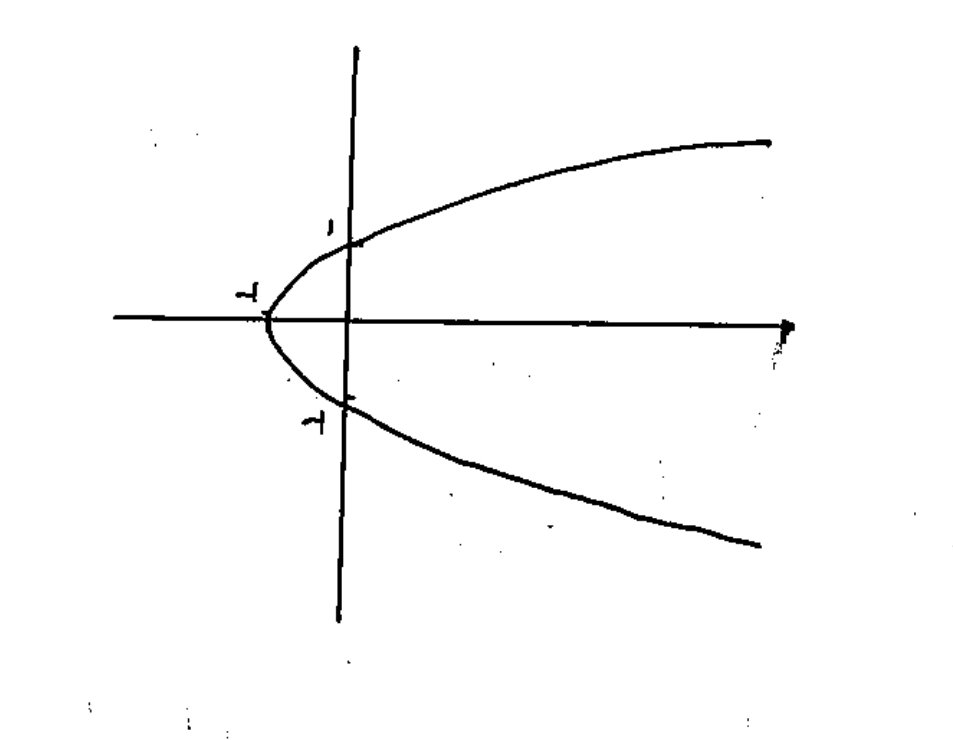
\includegraphics[width=1.8in,height=1.8in]{figures/ch07/figure1021_4.png}
	\caption{Feasible set of constraint 3} 
	%\label{fig:graph} 
\end{marginfigure}

Constraint 3:
\begin{equation*}
H_3=
\begin{bmatrix}
0 & 0\\
0 & 2
\end{bmatrix}
\qquad
c_3^{\trans} = 
\begin{bmatrix}
-1 & 0
\end{bmatrix}
\qquad
d_3 = -1 
\end{equation*}

So this constraint can be written as
$$x^2_2 - x_1 - 1\leq 0$$
The corresponding feasible set of this constraint is illustrated on r.h.s.


Put all these 3 constraints together(i.e., find the intersection of above 3 feasible sets), so we can obtain the desired feasible set for this QCQP problem
\begin{marginfigure}
	\centering
	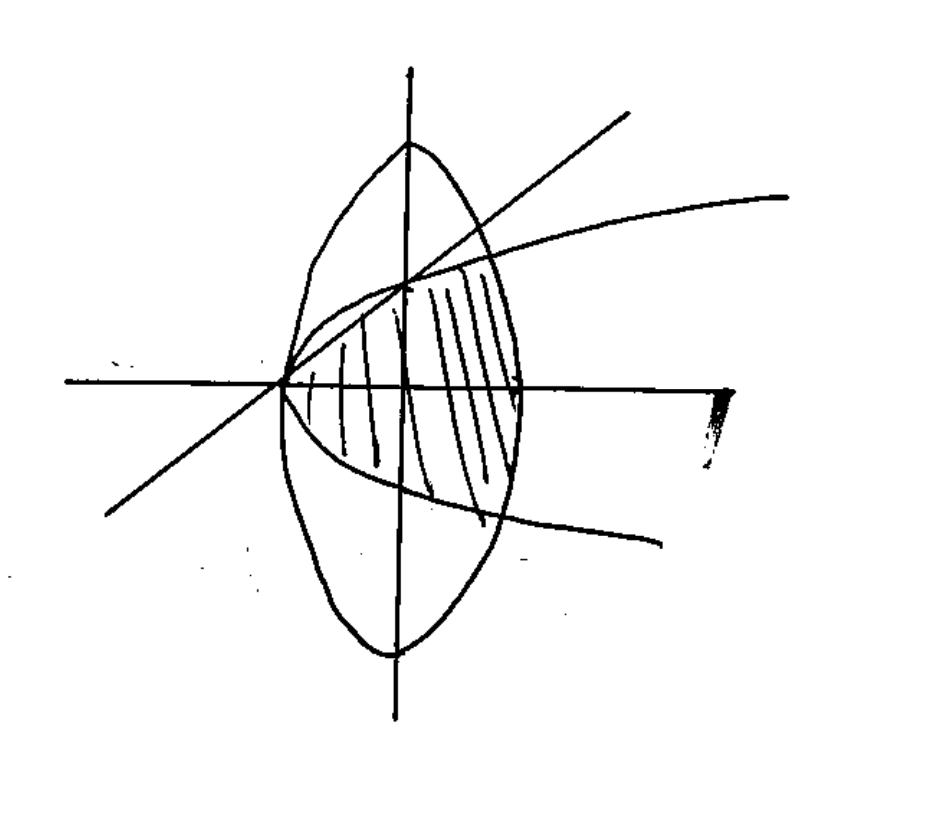
\includegraphics[width=1.8in,height=1.8in]{figures/ch07/figure1021_5.png}
	\caption{Feasible set for this QCQP} 
	%\label{fig:graph} 
\end{marginfigure}
\end{example}

